\documentclass[10pt,a4paper]{article}

\pdfoutput=1

% ── Encoding & Language ───────────────────────────────────────
\usepackage[T1]{fontenc}
\usepackage[utf8]{inputenc}
\usepackage[english]{babel}

% ── Page Layout ────────────────────────────────────────────────
\usepackage[margin=1in]{geometry}

% ── Math ──────────────────────────────────────────────────────
\usepackage{amsmath,amssymb,mathtools}

% ── Graphics & Figures ────────────────────────────────────────
\usepackage{graphicx}
\usepackage{float}

% ── Tables ────────────────────────────────────────────────────
\usepackage{booktabs}
\usepackage{multirow}
\usepackage{array}
\usepackage{longtable}
\usepackage{tabularx}

% ── TikZ ──────────────────────────────────────────────────────
\usepackage{tikz}
\usetikzlibrary{positioning,arrows.meta,shapes.geometric,calc,decorations.pathreplacing}

% ── Code Listings ─────────────────────────────────────────────
\usepackage{listings}
\lstset{
  basicstyle=\ttfamily\small,
  breaklines=true,
  frame=single,
  backgroundcolor=\color{gray!10},
  keywordstyle=\color{blue},
  commentstyle=\color{green!50!black},
  stringstyle=\color{red!70!black},
}

% ── Colors ────────────────────────────────────────────────────
\usepackage[dvipsnames,svgnames]{xcolor}

% ── Hyperlinks (LAST among setup packages) ────────────────────
\usepackage[colorlinks=true,linkcolor=blue,citecolor=green,urlcolor=purple]{hyperref}

% ── Other ─────────────────────────────────────────────────────
\usepackage{enumitem}

\title{\textbf{Foundational Concepts}\\[0.3em]
\large Technical Vocabulary for Intelligent Warranty Analysis Systems}
\author{}
\date{}

\begin{document}
\maketitle
\tableofcontents
\newpage

% ============================================================
% CHAPTER: Foundational Concepts
% ============================================================

\section{Machine Learning Algorithms}
\label{sec:ml-algorithms}

This section presents the core machine learning algorithms that underpin intelligent classification systems, from fundamental supervised learning to advanced ensemble methods and cascade architectures.

\subsection{Supervised Learning}
\label{sec:supervised-learning}

Supervised learning is the branch of machine learning in which a model learns a mapping function $f: \mathcal{X} \to \mathcal{Y}$ from a labelled dataset $\mathcal{D} = \{(x_i, y_i)\}_{i=1}^{n}$, where each input example $x_i \in \mathcal{X}$ is paired with a known output value $y_i \in \mathcal{Y}$. The objective is to find a function $\hat{f}$ from a hypothesis class $\mathcal{F}$ that minimises the expected loss over the data distribution:

\begin{equation}
\hat{f} = \arg\min_{f \in \mathcal{F}} \frac{1}{n} \sum_{i=1}^{n} L(f(x_i), y_i)
\label{eq:erm}
\end{equation}

where $L$ is a loss function that quantifies the penalty for incorrect predictions. The corresponding generalisation error is:

\begin{equation}
R(f) = \mathbb{E}_{(x,y) \sim \mathcal{D}}[L(f(x), y)]
\label{eq:gen-error}
\end{equation}

Supervised learning is distinguished from unsupervised learning (no labels) and reinforcement learning (feedback through rewards) by the presence of explicit labelled examples during training. The quality and quantity of labels directly influence model performance: insufficient labels lead to underfitting, while label noise can mislead the optimisation process.

\begin{figure}[H]
    \centering
    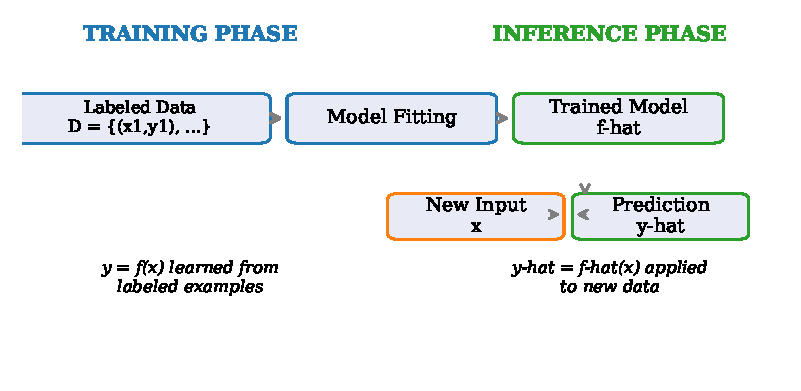
\includegraphics[width=0.85\textwidth]{figures/fig_supervised_learning_pipeline.pdf}
    \caption{Supervised learning pipeline: training and inference phases.}
    \label{fig:supervised-learning-pipeline}
\end{figure}

Supervised learning forms the foundation of classification and regression tasks in practical ML systems. In multi-output classification, where each input is assigned both a root-cause category and a decision label, supervised learning provides the mechanism by which patterns in the training data are generalised to unseen inputs.

\subsection{Multi-Class Classification}
\label{sec:multiclass-classification}

Multi-class classification extends binary classification to problems where the target variable $Y$ can take one of $K > 2$ discrete class labels: $Y \in \{c_1, c_2, \ldots, c_K\}$. Rather than producing a single probability, the model outputs a probability distribution over all $K$ classes:

\begin{equation}
P(y = c_k \mid x) = \frac{e^{z_k}}{\sum_{j=1}^{K} e^{z_j}}
\label{eq:softmax}
\end{equation}

where $z_k$ is the logit (unnormalised score) for class $k$. This softmax function ensures the outputs sum to unity and can be interpreted as probabilities. The corresponding loss function for multi-class classification is the cross-entropy loss:

\begin{equation}
L = -\sum_{k=1}^{K} y_k \log(\hat{y}_k)
\label{eq:ce-loss}
\end{equation}

where $y_k$ is the one-hot encoded true label and $\hat{y}_k = P(y = c_k \mid x)$ is the predicted probability for class $k$.

\begin{figure}[H]
    \centering
    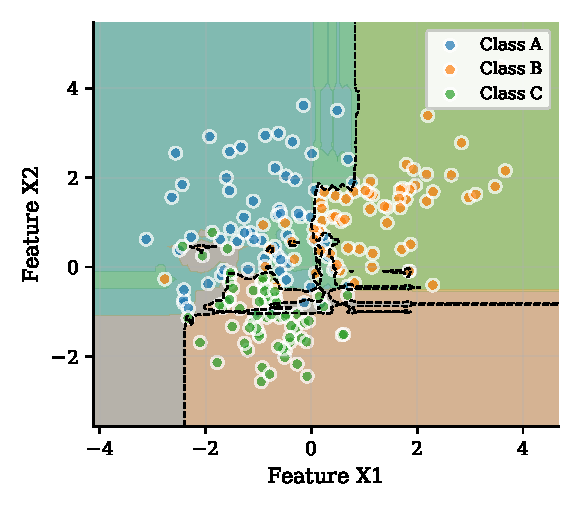
\includegraphics[width=0.8\textwidth]{figures/fig_multiclass_decision_boundary.pdf}
    \caption{Decision boundaries in a multi-class classification problem.}
    \label{fig:multiclass-decision-boundary}
\end{figure}

Multi-class classification is a fundamental paradigm for domains with more than two outcome categories. The probability vector produced by the softmax function also plays a structural role in cascade architectures (Section~\ref{sec:cascade-classification}), where the entire distribution over classes, rather than just the argmax prediction, is passed as features to a downstream classifier.

\subsection{Decision Trees}
\label{sec:decision-trees}

A decision tree is a hierarchical model that partitions the input space through a sequence of binary splits. Each internal node tests a single feature against a threshold $\theta$, and each leaf node holds a class label (for classification) or a numeric value (for regression). The tree is grown by recursively selecting the split that maximises an information-theoretic criterion.

The two most common split criteria for classification are Gini impurity and entropy (information gain). Gini impurity measures the probability of misclassifying a randomly chosen element if it were labelled according to the class distribution at that node:

\begin{equation}
G(\text{node}) = 1 - \sum_{k=1}^{K} p_k^2
\label{eq:gini}
\end{equation}

where $p_k$ is the proportion of class $k$ examples at the node. Entropy measures the information content of the class distribution:

\begin{equation}
H(\text{node}) = -\sum_{k=1}^{K} p_k \log_2(p_k)
\label{eq:entropy}
\end{equation}

The information gain for a candidate split $s$ that partitions a parent node into left and right children is:

\begin{equation}
IG(s) = H(\text{parent}) - \sum_{j \in \{\text{left}, \text{right}\}} \frac{N_j}{N} H(j)
\label{eq:info-gain}
\end{equation}

where $N$ is the number of examples at the parent node and $N_j$ is the number of examples in child $j$.

Splits that minimise Gini impurity (or equivalently maximise information gain) are preferred. A node is declared a leaf when a stopping criterion is met: maximum depth reached, fewer than \texttt{min\_samples\_split} examples remain, or no split improves purity. Decision trees are interpretable and require no feature scaling, but they overfit readily on training data. Both ensemble methods described next, Random Forest and XGBoost, address this limitation through fundamentally different strategies: bagging versus boosting.

\begin{figure}[H]
    \centering
    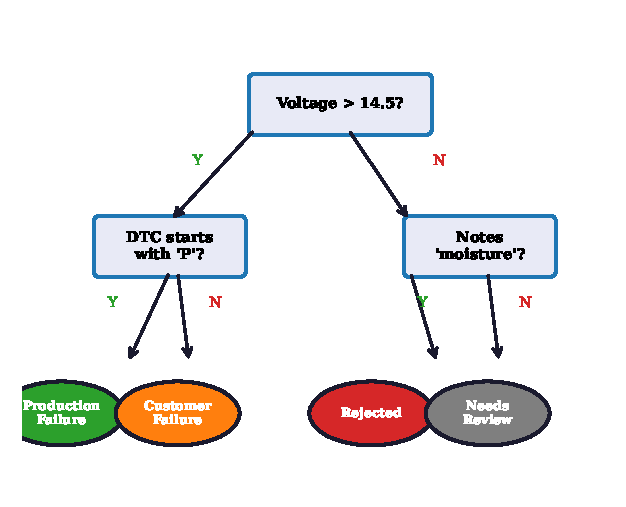
\includegraphics[width=0.85\textwidth]{figures/fig_decision_tree_example.pdf}
    \caption{A decision tree with feature tests at internal nodes and class labels at leaf nodes.}
    \label{fig:decision-tree-example}
\end{figure}

\subsection{Random Forest}
\label{sec:random-forest}

Random Forest is an ensemble method that reduces overfitting by training many decision trees independently and aggregating their predictions. Each tree is trained on a bootstrap sample of the data, and at each split only a random subset of features is considered. The final prediction is determined by majority vote across all trees.

\subsubsection{Bagging and Bootstrap Aggregation}

Bagging (Bootstrap Aggregation) trains each tree on an independently drawn bootstrap sample of the original dataset. A bootstrap sample is formed by sampling $n$ rows from the training set with replacement, where $n$ is the original dataset size. The probability that a specific row is \emph{not} selected in any single draw from $n$ draws is:

\begin{equation}
P(\text{not selected}) = \left(1 - \frac{1}{n}\right)^n \xrightarrow{n \to \infty} e^{-1} \approx 0.368
\label{eq:oob-prob}
\end{equation}

On average, approximately 63.2\% of unique rows appear in any given bootstrap sample; the remaining 36.8\% are ``out-of-bag'' (OOB) and can be used for internal validation without a separate validation set. For classification, the final prediction is the majority vote across all trees:

\begin{equation}
\hat{y} = \arg\max_{k} \sum_{t=1}^{T} \mathbb{I}(\hat{y}_t = c_k)
\label{eq:rf-vote}
\end{equation}

where $T$ is the number of trees, $\hat{y}_t$ is the prediction of tree $t$, and $\mathbb{I}(\cdot)$ is the indicator function.

\subsubsection{Random Feature Subsampling}

At each node split during tree construction, only a random subset of $m$ features is considered as candidates for the best split. This decorrelates the trees: even if one feature is highly predictive, it will not dominate every tree. The standard recommendation for classification is:

\begin{equation}
m = \lfloor \sqrt{p} \rfloor
\label{eq:rf-features}
\end{equation}

where $p$ is the total number of features. Feature subsampling ensures that different trees specialise in different parts of the feature space, increasing diversity and reducing ensemble variance.

\begin{figure}[H]
    \centering
    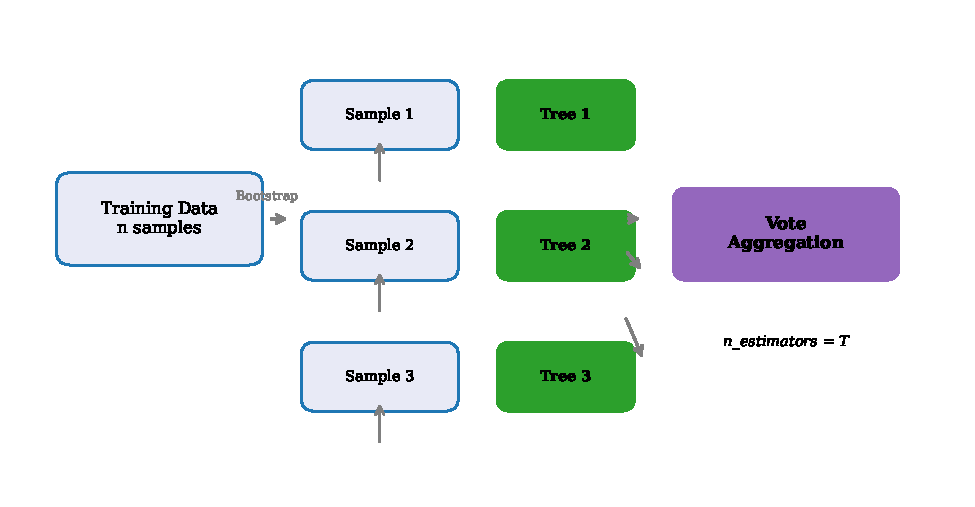
\includegraphics[width=0.85\textwidth]{figures/fig_random_forest_architecture.pdf}
    \caption{Random Forest: bootstrap sampling, independent tree training, and majority vote aggregation.}
    \label{fig:random-forest-architecture}
\end{figure}

Aggregating over many trees that were trained on different bootstrap samples reduces variance without significantly increasing bias, the key trade-off that makes Random Forest a robust general-purpose classifier.

\subsection{XGBoost / Gradient Boosting}
\label{sec:xgboost}

Gradient boosting is an ensemble method that builds trees \emph{sequentially}: each new tree is trained to correct the residual errors of the combined ensemble so far. Formally, let $F_t(x)$ be the ensemble prediction after $t$ trees. The $(t+1)$-th tree $h_{t+1}(x)$ is fitted to the negative gradient of the loss function evaluated at $F_t(x)$:

\begin{equation}
h_{t+1} = \arg\min_{h} \sum_{i=1}^{n} L\left(y_i, F_t(x_i) + h(x_i)\right)
\label{eq:boost-objective}
\end{equation}

The ensemble is updated by:

\begin{equation}
F_{t+1}(x) = F_t(x) + \eta \cdot h_{t+1}(x)
\label{eq:boost-update}
\end{equation}

where $\eta$ is the learning rate (also called shrinkage), a small positive constant that controls the contribution of each tree. A low learning rate (e.g., 0.02) requires more trees but typically yields better generalisation.

The key distinction from Random Forest (Section~\ref{sec:random-forest}) is that gradient boosting trees are \textbf{additive} (each tree corrects the ensemble's remaining error) rather than \textbf{independent} (each tree votes). This makes boosting more prone to overfitting if unregularised, but also more powerful when properly tuned.

XGBoost (eXtreme Gradient Boosting) extends traditional gradient boosting with a regularised objective function:

\begin{equation}
\mathcal{L}(\theta) = \sum_{i=1}^{n} L(y_i, \hat{y}_i) + \sum_{k=1}^{T} \left(\gamma T_k + \frac{1}{2}\lambda \sum_{j=1}^{T_k} w_j^2 + \alpha \sum_{j=1}^{T_k} |w_j|\right)
\label{eq:xgb-objective}
\end{equation}

where $T_k$ is the number of leaves in tree $k$, $w_j$ are the leaf weights, $\gamma$ is the minimum split loss (a pruning parameter), $\lambda$ is the L2 regularisation coefficient on leaf weights, and $\alpha$ is the L1 regularisation coefficient. These regularisation terms directly penalise complex trees and large leaf weights, reducing overfitting.

XGBoost further optimises training through a second-order Taylor approximation of the loss function:

\begin{equation}
\mathcal{L}^{(t)} \approx \sum_{i=1}^{n} \left[g_i h_t(x_i) + \frac{1}{2} h_i h_t^2(x_i)\right] + \Omega(h_t)
\label{eq:xgb-taylor}
\end{equation}

where $g_i = \partial_{\hat{y}^{(t-1)}} L(y_i, \hat{y}^{(t-1)})$ is the first-order gradient and $h_i = \partial^2_{\hat{y}^{(t-1)}} L(y_i, \hat{y}^{(t-1)})$ is the second-order gradient (Hessian). Using both first and second derivatives enables more accurate split finding and faster convergence than first-order methods alone.

\begin{figure}[H]
    \centering
    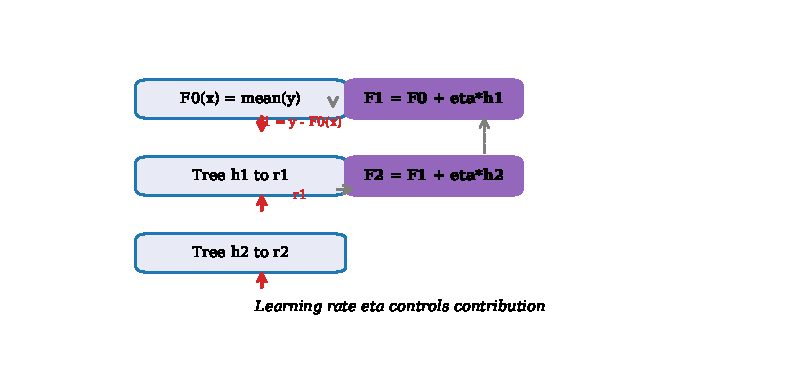
\includegraphics[width=0.85\textwidth]{figures/fig_gradient_boosting_sequential.pdf}
    \caption{Gradient boosting: each successive tree is fitted to the residuals of the current ensemble.}
    \label{fig:gradient-boosting-sequential}
\end{figure}

XGBoost represents the state-of-the-art for structured/tabular data classification. Its combination of second-order optimisation, built-in regularisation, and efficient handling of sparse features makes it superior to Random Forest on datasets with mixed feature types, such as combinations of TF-IDF vectors and one-hot encoded categoricals.

\subsection{Cascade / Stacked Classification}
\label{sec:cascade-classification}

A cascade (or stacked) classification architecture is a multi-stage pipeline where the output, typically a probability vector, of a first-stage classifier is concatenated with the original features and used as input to a second-stage classifier. The key insight is that the downstream decision causally depends on the upstream classification: knowing \emph{what} went wrong (failure analysis) informs \emph{whether} the warranty should be approved (warranty decision).

Let $x$ denote the original feature vector and $f_1$ the first-stage classifier. The first-stage prediction is the full probability vector over all classes:

\begin{equation}
\mathbf{p}^{(1)} = \text{softmax}(f_1(x))
\label{eq:cascade-stage1}
\end{equation}

The augmented feature vector for the second-stage classifier $f_2$ is:

\begin{equation}
x' = [x \mid \mathbf{p}^{(1)}]
\label{eq:cascade-augment}
\end{equation}

where $[\cdot \mid \cdot]$ denotes horizontal concatenation. The final prediction is:

\begin{equation}
\hat{y} = \arg\max_k f_2(x')_k
\label{eq:cascade-stage2}
\end{equation}

\begin{figure}[H]
    \centering
    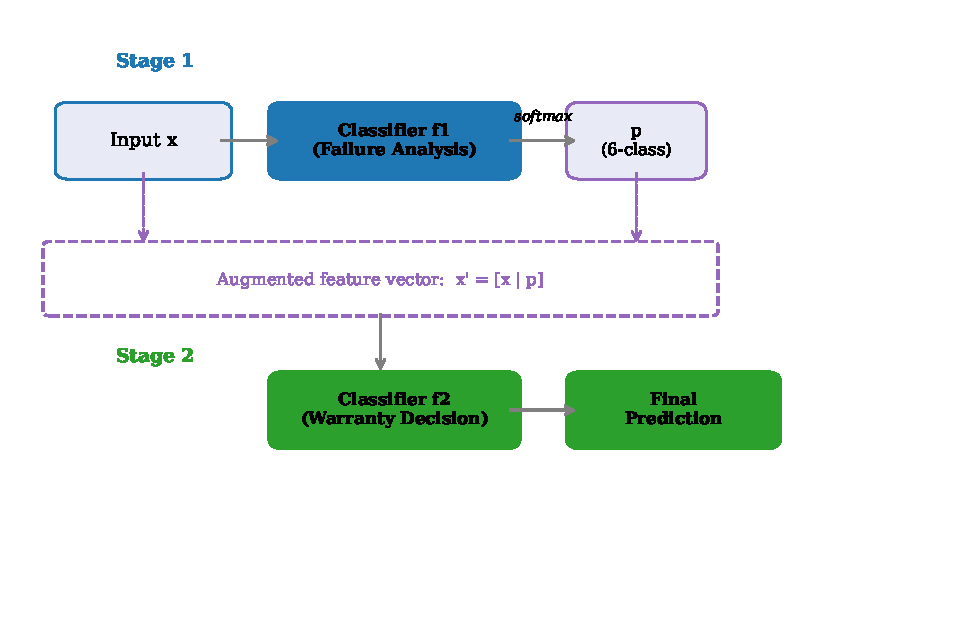
\includegraphics[width=0.85\textwidth]{figures/fig_cascade_classifier.pdf}
    \caption{Cascade classification: first-stage probabilities augment the feature vector for the second-stage classifier.}
    \label{fig:cascade-classifier}
\end{figure}

A critical implementation detail is the use of out-of-fold (OOF) probabilities during training (Section~\ref{sec:cross-validation}). Naively training the first-stage classifier on all training data and then using its in-sample probabilities to train the second-stage classifier would introduce data leakage, since the first-stage model would ``know'' the training examples too well. Using OOF probabilities ensures that the probability vectors passed to the second stage come from held-out folds, preventing overconfident cascade features.

\subsection{Cross-Validation and Out-of-Fold Predictions}
\label{sec:cross-validation}

K-fold cross-validation partitions the training data $\mathcal{D}$ into $K$ equal (or approximately equal) folds:

\begin{equation}
\mathcal{D} = \bigcup_{k=1}^{K} \mathcal{D}_k, \quad \mathcal{D}_j \cap \mathcal{D}_k = \emptyset \text{ for } j \neq k
\label{eq:kfold}
\end{equation}

The model is trained $K$ times, each time using $K-1$ folds for training and the held-out fold for validation. This produces $K$ performance estimates that can be averaged for a robust evaluation.

Out-of-fold (OOF) predictions extend cross-validation to produce unbiased probability estimates for each training example. For example $i \in \mathcal{D}_k$, the OOF prediction is:

\begin{equation}
\hat{y}_i^{\text{OOF}} = f_{\theta_{-k}}(x_i), \quad \text{where } \theta_{-k} \text{ is trained on } \mathcal{D} \setminus \mathcal{D}_k
\label{eq:oof}
\end{equation}

\begin{figure}[H]
    \centering
    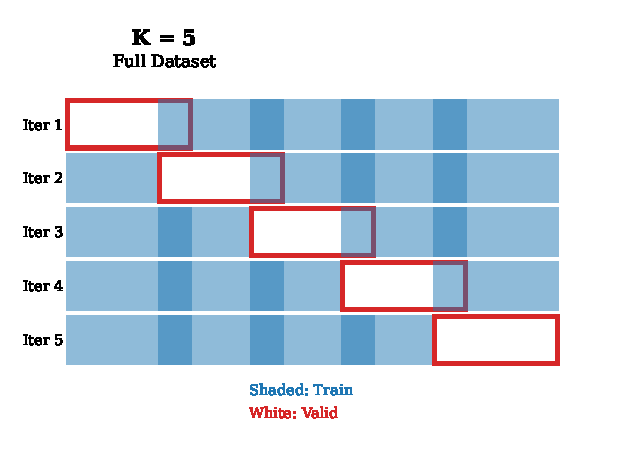
\includegraphics[width=0.85\textwidth]{figures/fig_kfold_cross_validation.pdf}
    \caption{K-fold cross-validation: each fold serves as the validation set exactly once.}
    \label{fig:kfold-cross-validation}
\end{figure}

OOF predictions are essential for cascade architectures because they provide probability vectors that were generated by models that did not ``see'' the corresponding examples during training, eliminating the data leakage that would arise from using in-sample predictions.

\subsection{Train-Test Split and Data Leakage Prevention}
\label{sec:train-test-split}

The train-test split partitions the available data into disjoint training and test sets. The test set is held out until final evaluation to provide an unbiased estimate of generalisation performance. A stratified split preserves the class distribution across both sets:

\begin{equation}
\frac{| \{i \in \mathcal{D}_{\text{train}} : y_i = c_k\} |}{|\mathcal{D}_{\text{train}}|} \approx \frac{| \{i \in \mathcal{D}_{\text{test}} : y_i = c_k\} |}{|\mathcal{D}_{\text{test}}|} \quad \forall k
\label{eq:stratified-split}
\end{equation}

Data leakage occurs when information from the test set inadvertently influences the training process, leading to inflated evaluation metrics. Common sources include:

\begin{itemize}
    \item Fitting preprocessing transformers (scalers, encoders, vectorisers) on the full dataset before splitting
    \item Using future information as features (temporal leakage)
    \item Including test samples in the training set through duplicate entries
\end{itemize}

\begin{figure}[H]
    \centering
    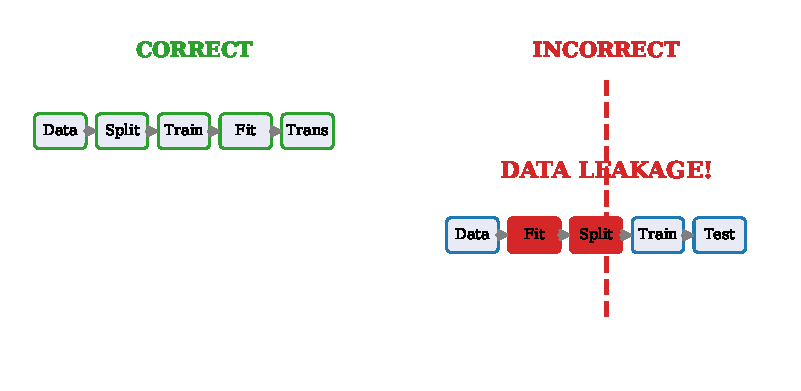
\includegraphics[width=0.85\textwidth]{figures/fig_data_leakage_scenarios.pdf}
    \caption{Data leakage scenarios: correct vs.\ incorrect preprocessing pipelines.}
    \label{fig:data-leakage-scenarios}
\end{figure}

The correct practice is to fit all transformers exclusively on the training split and then apply the fitted transformations to the test split. This ensures that no information from the test set leaks into model training or feature engineering.

% ============================================================
\section{Feature Engineering}
\label{sec:feature-engineering}

Feature engineering transforms raw data into numerical representations suitable for machine learning models. The quality of features directly determines the upper bound of model performance, a principle often summarised as ``garbage in, garbage out.''

\subsection{TF-IDF Vectorisation}
\label{sec:tfidf}

Term Frequency--Inverse Document Frequency (TF-IDF) converts text documents into numerical vectors by weighting each term by its frequency in the document and its rarity across the corpus. It is the primary mechanism for converting raw text into a fixed-length feature vector.

\textbf{Term Frequency (TF)} measures how often a term $t$ appears in document $d$:

\begin{equation}
TF(t, d) = \frac{\text{count of term } t \text{ in } d}{\text{total terms in } d}
\label{eq:tf}
\end{equation}

\textbf{Inverse Document Frequency (IDF)} measures how rare a term is across the corpus $\mathcal{D}$:

\begin{equation}
IDF(t, \mathcal{D}) = \log\left(\frac{1 + |\mathcal{D}|}{1 + df(t)}\right) + 1
\label{eq:idf}
\end{equation}

where $|\mathcal{D}|$ is the total number of documents and $df(t)$ is the number of documents containing term $t$. The additive smoothing ($+1$ in both numerator and denominator) prevents division by zero for terms unseen in the corpus. The final TF-IDF score is the product:

\begin{equation}
TF\text{-}IDF(t, d, \mathcal{D}) = TF(t, d) \times IDF(t, \mathcal{D})
\label{eq:tfidf}
\end{equation}

\begin{figure}[H]
    \centering
    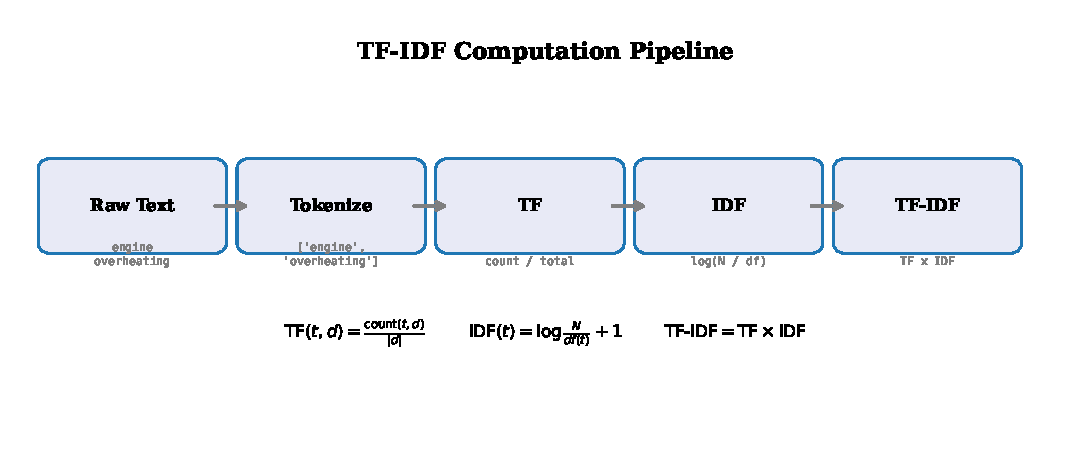
\includegraphics[width=0.85\textwidth]{figures/fig_tfidf_computation.pdf}
    \caption{TF-IDF computation pipeline: raw text $\rightarrow$ tokenisation $\rightarrow$ TF $\rightarrow$ IDF weighting $\rightarrow$ sparse vector.}
    \label{fig:tfidf-computation}
\end{figure}

TF-IDF is the standard baseline for text classification tasks. It captures term importance while down-weighting ubiquitous terms (such as ``the'' or ``is'') that appear in every document and therefore carry little discriminative information. The resulting vectors are typically high-dimensional and sparse (most entries are zero), which motivates the use of sparse matrix representations (Section~\ref{sec:sparse-matrices}).

\subsection{One-Hot Encoding}
\label{sec:one-hot-encoding}

One-hot encoding (OHE) converts a categorical variable with $K$ distinct values into a binary vector of length $K$, where exactly one element is 1 (the ``hot'' element) and all others are 0:

\begin{equation}
\text{OHE}(c_j) = [0, \ldots, 0, \underbrace{1}_{j\text{-th position}}, 0, \ldots, 0] \in \{0, 1\}^K
\label{eq:ohe}
\end{equation}

One-hot encoding preserves the nominal nature of categorical data: no ordinal relationship is implied between categories. However, it increases dimensionality, especially for high-cardinality categorical features, and produces sparse vectors.

\begin{figure}[H]
    \centering
    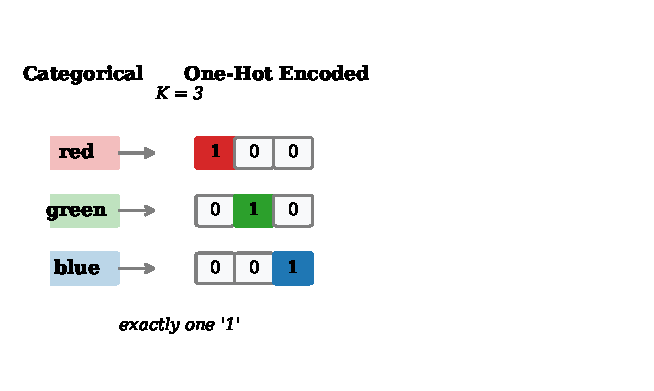
\includegraphics[width=0.8\textwidth]{figures/fig_one_hot_encoding.pdf}
    \caption{One-hot encoding maps categorical values to sparse binary vectors.}
    \label{fig:one-hot-encoding}
\end{figure}

One-hot encoding enables ML models to process nominal categorical variables without imposing ordinal relationships. It is commonly applied to features such as customer complaint categories, supplier identifiers, and binned numeric ranges.

\subsection{Feature Scaling / Standardisation}
\label{sec:feature-scaling}

Standardisation (z-score normalisation) transforms continuous features to have zero mean and unit variance:

\begin{equation}
z = \frac{x - \mu_{\text{train}}}{\sigma_{\text{train}}}
\label{eq:zscore}
\end{equation}

where $\mu_{\text{train}} = \frac{1}{n}\sum_{i=1}^{n} x_i$ and $\sigma_{\text{train}} = \sqrt{\frac{1}{n}\sum_{i=1}^{n}(x_i - \mu_{\text{train}})^2}$ are computed exclusively on the training set. Applying training statistics to the test set prevents data leakage (Section~\ref{sec:train-test-split}).

\begin{figure}[H]
    \centering
    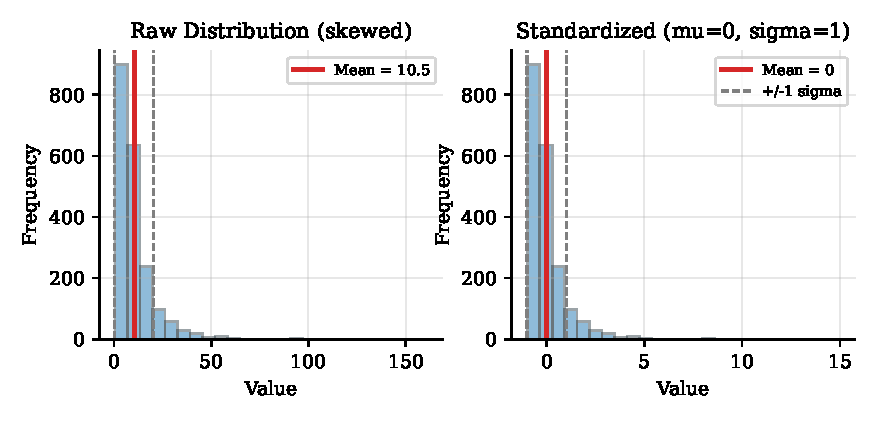
\includegraphics[width=0.8\textwidth]{figures/fig_feature_scaling_comparison.pdf}
    \caption{Effect of standardisation: raw distribution (left) vs.\ standardised distribution (right).}
    \label{fig:feature-scaling-comparison}
\end{figure}

Standardisation is critical for gradient-based optimisation (which converges faster on centred features), distance-based algorithms (which are sensitive to feature scales), and regularisation (which penalises large weights disproportionately on unscaled features).

\subsection{Label Encoding}
\label{sec:label-encoding}

Label encoding maps categorical class labels to integer values:

\begin{equation}
\text{LabelEncode}(c_j) = j, \quad j \in \{0, 1, \ldots, K-1\}
\label{eq:label-encode}
\end{equation}

Unlike one-hot encoding, label encoding produces a single integer column. The integer mapping itself carries no ordinal meaning for the model; it is primarily a required interface for classification algorithms that expect integer targets. Label encoding is typically used for the target variable, while one-hot encoding (Section~\ref{sec:one-hot-encoding}) is used for input features.

\subsection{Feature Binning / Discretisation}
\label{sec:feature-binning}

Feature binning (discretisation) converts a continuous variable into discrete categories by partitioning its range into intervals. Equal-width binning divides the range $\left[x_{\min}, x_{\max}\right]$ into $K$ bins of equal size:

\begin{equation}
\text{bin}(x) = \left\lfloor \frac{x - x_{\min}}{x_{\max} - x_{\min}} \times K \right\rfloor
\label{eq:binning}
\end{equation}

Quantile-based binning (also called equal-frequency binning) assigns approximately $n/K$ samples to each bin, ensuring balanced class representation across bins.

\begin{figure}[H]
    \centering
    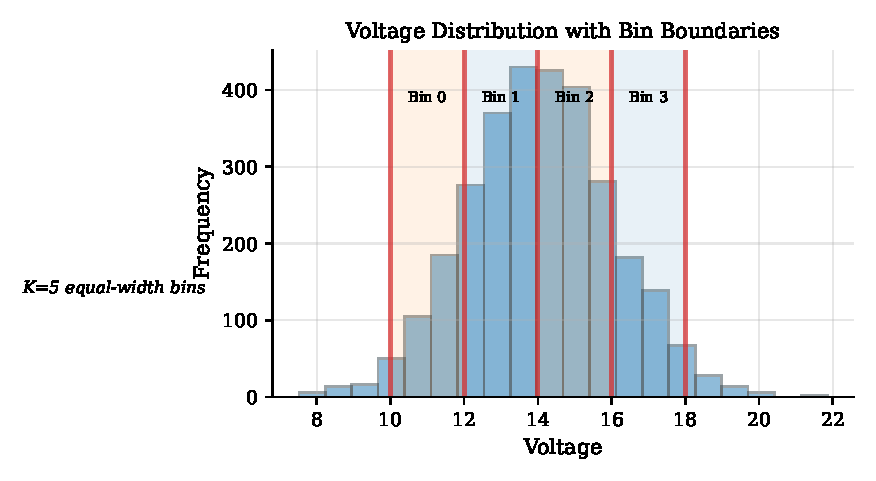
\includegraphics[width=0.8\textwidth]{figures/fig_feature_binning.pdf}
    \caption{Feature binning: continuous values mapped to categorical bins.}
    \label{fig:feature-binning}
\end{figure}

Binning captures domain-specific thresholds that linear models cannot represent directly. For example, a voltage reading of 16.1V may be qualitatively different from 14.0V, and binning separates these into distinct categories (``extreme'' vs.\ ``normal'') that capture this domain knowledge.

\subsection{Interaction Features}
\label{sec:interaction-features}

Interaction features are created by combining two or more existing features to capture joint effects that individual features cannot represent. A multiplicative interaction between two features is:

\begin{equation}
x_{\text{interaction}} = x_i \times x_j
\label{eq:interaction-mult}
\end{equation}

A binary (logical AND) interaction tests whether two conditions hold simultaneously:

\begin{equation}
x_{\text{interaction}} = \mathbb{I}(x_i > \tau_i \land x_j = 1)
\label{eq:interaction-binary}
\end{equation}

A polynomial expansion of degree 2 generates all pairwise (and optionally squared) terms:

\begin{equation}
\phi(x) = [x_1, x_2, \ldots, x_p, x_1x_2, x_1x_3, \ldots, x_{p-1}x_p]
\label{eq:polynomial}
\end{equation}

\begin{figure}[H]
    \centering
    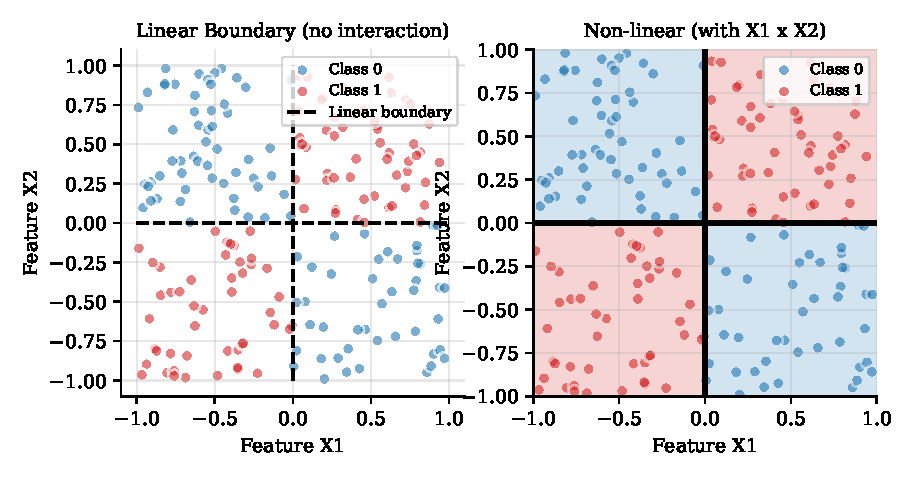
\includegraphics[width=0.8\textwidth]{figures/fig_interaction_features.pdf}
    \caption{Interaction features enable non-linear decision boundaries.}
    \label{fig:interaction-features}
\end{figure}

Interaction features enable linear models to capture non-linear relationships. Tree-based models can learn interactions implicitly through successive splits, but explicit interaction features can accelerate learning and improve interpretability.

\subsection{Sparse Matrix Operations}
\label{sec:sparse-matrices}

Compressed Sparse Row (CSR) format stores a sparse matrix using three one-dimensional arrays: \texttt{data} (non-zero values), \texttt{indices} (column indices of each non-zero), and \texttt{indptr} (row pointers). For a matrix with $N$ non-zero entries and $m$ rows, the storage requirement is:

\begin{equation}
\text{Memory}_{\text{CSR}} = N \times (\text{sizeof(data)} + \text{sizeof(indices)}) + (m+1) \times \text{sizeof(indptr)}
\label{eq:csr-memory}
\end{equation}

Compared to dense storage, which requires $m \times n \times \text{sizeof(element)}$, CSR format offers dramatic savings when the sparsity ratio $N/(m \times n)$ is small. For a TF-IDF matrix with 100,000 documents and 40 features where most documents contain only a handful of DTC terms, the sparsity ratio can exceed 90\%.

\begin{figure}[H]
    \centering
    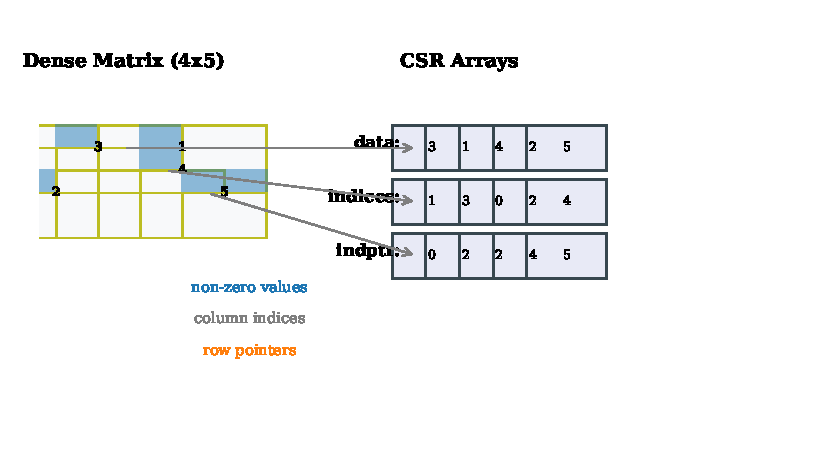
\includegraphics[width=0.8\textwidth]{figures/fig_csr_format.pdf}
    \caption{CSR sparse matrix format: dense matrix decomposed into \texttt{data}, \texttt{indices}, and \texttt{indptr} arrays.}
    \label{fig:csr-format}
\end{figure}

Sparse matrix representations are essential for memory-efficient storage of TF-IDF vectors and one-hot encoded features, which are predominantly zero. Horizontal stacking (\texttt{hstack}) of sparse matrices enables the efficient combination of multiple feature types (TF-IDF, OHE, numeric) into a single design matrix.

\subsection{Regular Expression Pattern Matching}
\label{sec:regex}

Regular expressions (regex) define search patterns using a formal syntax of literals, metacharacters, and quantifiers, enabling structured extraction from unstructured text. A regular expression $r$ matches a string $s$ if the pattern occurs as a substring:

\begin{equation}
\text{match}(s, r) = \begin{cases} \text{true} & \text{if } s \text{ contains a substring matching } r \\ \text{false} & \text{otherwise} \end{cases}
\label{eq:regex-match}
\end{equation}

Common regex patterns for extracting structured identifiers from free text include:

\begin{itemize}
    \item Automotive Diagnostic Trouble Codes: \texttt{\textbackslash b[PUCB][0-9A-Fa-f]\{4\}\textbackslash b}
    \item Numeric voltage values: \texttt{\textbackslash b[0-9]+\textbackslash.?[0-9]*\textbackslash bV?}
    \item Date patterns: \texttt{[0-9]\{4\}-[0-9]\{2\}-[0-9]\{2\}}
\end{itemize}

Regular expressions provide a fast, deterministic mechanism for extracting structured identifiers from free-text fields such as technician notes and log files. They serve as a complement to probabilistic NLP methods, offering perfect precision when the pattern is well-defined.

\subsection{Keyword-Based Text Classification}
\label{sec:keyword-classification}

Keyword-based text classification maps input text to a category by checking for the presence of predefined keywords, typically using a first-match-wins strategy. Formally, given an ordered list of keyword-category pairs $\{(k_1, c_1), (k_2, c_2), \ldots, (k_m, c_m)\}$, the classification function is:

\begin{equation}
\text{classify}(t) = c_j \quad \text{where } j = \min\{i : \exists k \in \mathcal{K}_i, k \subseteq \text{lowercase}(t)\}
\label{eq:keyword-classify}
\end{equation}

where $\mathcal{K}_i$ is the keyword set for category $i$ and $j$ is the smallest index for which any keyword in $\mathcal{K}_i$ is found as a substring of the lowercased input text $t$.

Keyword classification is fast, interpretable, and deterministic. It serves as a reliable baseline when labelled training data is scarce or when deterministic behaviour is required. Its limitations include sensitivity to vocabulary differences (the keyword list must cover all relevant terms) and inability to capture semantic similarity between terms with different spellings.

\subsection{Fuzzy String Matching}
\label{sec:fuzzy-matching}

Fuzzy string matching measures similarity between strings when they are not identical, accounting for character insertions, deletions, substitutions, and transpositions. The Levenshtein (edit) distance between two strings $a$ and $b$ is the minimum number of single-character edits required to transform $a$ into $b$:

\begin{equation}
\text{lev}(a, b) = \begin{cases}
|a| & \text{if } |b| = 0 \\
|b| & \text{if } |a| = 0 \\
\text{lev}(a', b') & \text{if } a_{|a|} = b_{|b|} \\
1 + \min\begin{cases} \text{lev}(a', b) \\
\text{lev}(a, b') \\
\text{lev}(a', b') \end{cases} & \text{otherwise}
\end{cases}
\label{eq:levenshtein}
\end{equation}

where $a'$ denotes $a$ with its last character removed. The normalised similarity ratio is:

\begin{equation}
\text{similarity}(a, b) = 1 - \frac{\text{lev}(a, b)}{\max(|a|, |b|)}
\label{eq:similarity-ratio}
\end{equation}

\begin{figure}[H]
    \centering
    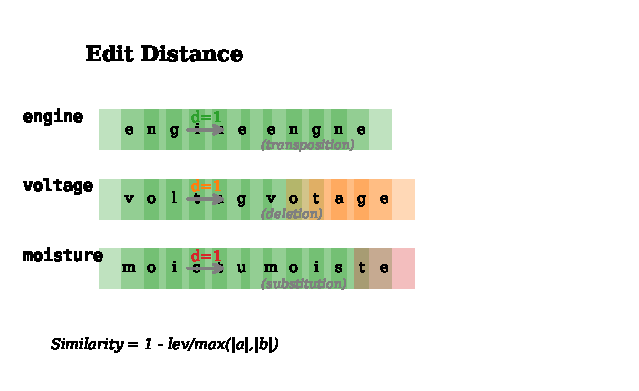
\includegraphics[width=0.8\textwidth]{figures/fig_fuzzy_matching.pdf}
    \caption{Fuzzy string matching: edit distance between similar strings.}
    \label{fig:fuzzy-matching}
\end{figure}

Fuzzy string matching handles typos, abbreviations, and variant spellings in free-text fields. It is commonly used as a fallback after keyword matching fails, providing a ``closest match'' from a known vocabulary based on a similarity threshold.

% ============================================================
\section{Rule-Based Systems}
\label{sec:rule-based-systems}

Rule-based systems encode domain expertise as explicit logical rules, providing transparent and deterministic decisions. They complement statistical models by handling high-confidence edge cases where pattern matching is more reliable than probabilistic prediction.

\subsection{Deterministic Rule Engines}
\label{sec:rule-engines}

A rule-based system (rule engine) encodes domain knowledge as a collection of IF--THEN rules, where each rule specifies a condition (a predicate over input values) and a consequence (an action or output to produce when the condition is satisfied). Formally:

\begin{equation}
R_j: \text{IF } \phi_j(x) \text{ THEN } \text{output} = o_j
\label{eq:rule-structure}
\end{equation}

where $\phi_j: \mathcal{X} \to \{\text{true}, \text{false}\}$ is a boolean predicate over the input features and $o_j$ is the associated output (class label, confidence score, and reason string).

The rule set is evaluated in a fixed priority order, and the first rule whose condition evaluates to true fires:

\begin{equation}
\text{output}(x) = o_j \quad \text{where } j = \min\{i : \phi_i(x) = \text{true}\}
\label{eq:rule-eval}
\end{equation}

If no rule fires, a default fallback mechanism produces the output.

\begin{figure}[H]
    \centering
    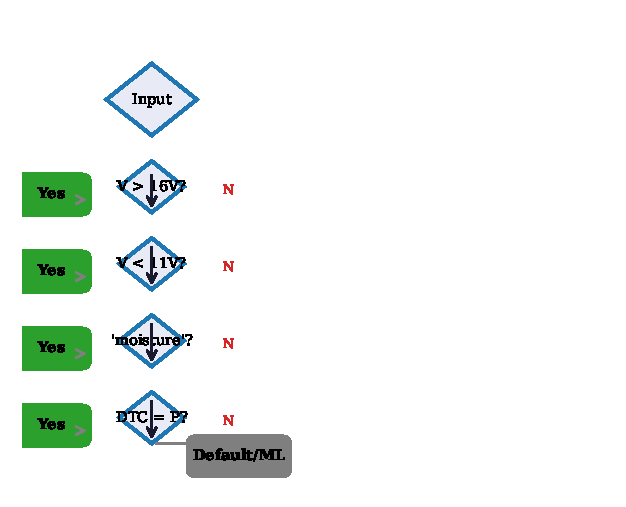
\includegraphics[width=0.85\textwidth]{figures/fig_rule_engine_flow.pdf}
    \caption{Deterministic rule engine: rules evaluated in priority order; first match fires.}
    \label{fig:rule-engine-flow}
\end{figure}

Rule engines provide transparent, auditable decisions for high-confidence edge cases. Their advantages include full interpretability (the fired rule explains the decision), deterministic reproducibility (same input always produces the same output), and ease of maintenance (new rules can be added without retraining).

\subsection{First-Match-Wins Evaluation Strategy}
\label{sec:first-match-wins}

The first-match-wins strategy evaluates rules in a fixed priority order, returning the output of the first rule whose condition is satisfied:

\begin{equation}
\text{result}(x) = \begin{cases}
o_1 & \text{if } \phi_1(x) \\
o_2 & \text{if } \neg\phi_1(x) \land \phi_2(x) \\
\vdots & \\
o_m & \text{if } \bigwedge_{i=1}^{m-1} \neg\phi_i(x) \land \phi_m(x) \\
\text{default} & \text{if } \bigwedge_{i=1}^{m} \neg\phi_i(x)
\end{cases}
\label{eq:first-match}
\end{equation}

This evaluation order encodes domain confidence: the most reliable rules (e.g., voltage thresholds based on direct measurements) are evaluated first, while lower-confidence rules (e.g., DTC prefix heuristics) are evaluated last. The strategy ensures deterministic, reproducible outcomes and makes the priority order itself a form of domain knowledge engineering.

\subsection{Confidence Thresholding}
\label{sec:confidence-thresholding}

Confidence thresholding maps continuous confidence scores to discrete decision categories using fixed threshold boundaries. A three-tier system classifies decisions into firm, cautious, and manual review categories:

\begin{equation}
\text{status}(c) = \begin{cases}
\text{Firm} & \text{if } c \geq \tau_{\text{firm}} \\
\text{Cautious} & \text{if } \tau_{\text{manual}} \leq c < \tau_{\text{firm}} \\
\text{Manual Review} & \text{if } c < \tau_{\text{manual}}
\end{cases}
\label{eq:thresholding}
\end{equation}

where $\tau_{\text{firm}}$ (e.g., 85\%) and $\tau_{\text{manual}}$ (e.g., 65\%) are domain-calibrated thresholds. Additionally, raw confidence scores are clamped to a valid range to prevent unrealistic extreme values:

\begin{equation}
c_{\text{clamped}} = \min(c_{\max}, \max(c_{\min}, c_{\text{raw}}))
\label{eq:clamping}
\end{equation}

\begin{figure}[H]
    \centering
    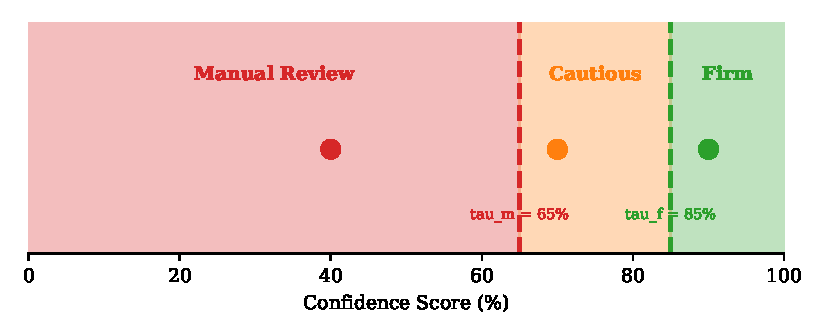
\includegraphics[width=0.85\textwidth]{figures/fig_confidence_thresholds.pdf}
    \caption{Confidence threshold regions mapping scores to decision categories.}
    \label{fig:confidence-thresholds}
\end{figure}

Confidence thresholding serves as a safety mechanism that routes uncertain predictions to human review, balancing automation efficiency with decision quality. The choice of thresholds should be calibrated on held-out validation data to ensure that the ``Firm'' category achieves the desired precision level while the ``Manual Review'' category captures the vast majority of uncertain cases.

% ============================================================
\section{Score Combination and Decision Fusion}
\label{sec:score-combination}

Intelligent decision systems often combine outputs from multiple independent sources, each offering a different perspective on the same input. This section presents the mathematical foundations for blending these signals into a unified, calibrated decision.

\subsection{Weighted Score Blending}
\label{sec:weighted-blending}

Weighted score blending combines confidence scores from multiple independent sources (rule engine, ML model, LLM) using a weighted linear combination, where the weights reflect the relative reliability of each source:

\begin{equation}
c_{\text{combined}} = \sum_{i=1}^{m} w_i \cdot c_i, \quad \text{subject to } \sum_{i=1}^{m} w_i = 1
\label{eq:weighted-blending}
\end{equation}

The weights can be context-dependent. When two sources agree on their prediction, higher combined confidence is warranted, encouraging an agreement bonus:

\begin{equation}
c_{\text{combined}} = w_{\text{rule}} \cdot c_{\text{rule}} + w_{\text{ml}} \cdot c_{\text{ml}} + b_{\text{agree}} \cdot \mathbb{I}(\text{rule agrees with ML})
\label{eq:agreement-bonus}
\end{equation}

where $b_{\text{agree}}$ is a fixed bonus added when the rule engine and ML model produce the same class label. Furthermore, when sources disagree, the weights are adjusted to reflect reduced confidence:

\begin{equation}
w_{\text{rule}} = \begin{cases} w_{\text{rule}}^{\text{agree}} & \text{if sources agree} \\ w_{\text{rule}}^{\text{disagree}} & \text{if sources disagree} \end{cases}
\label{eq:conditional-weights}
\end{equation}

\begin{figure}[H]
    \centering
    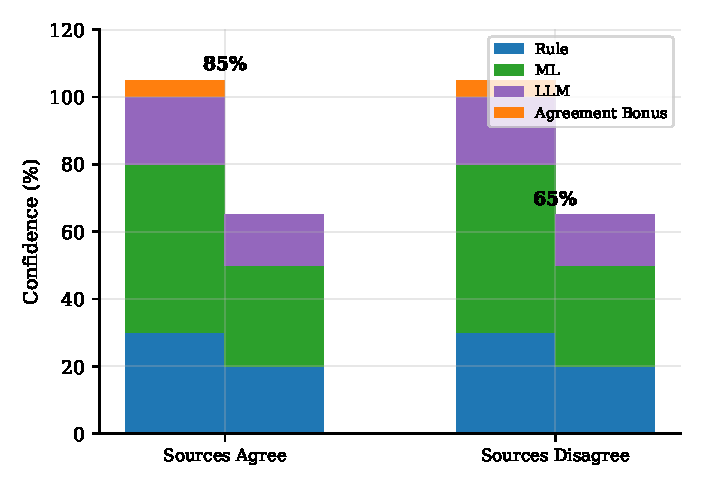
\includegraphics[width=0.85\textwidth]{figures/fig_weighted_blending.pdf}
    \caption{Weighted score blending: contributions from multiple decision sources.}
    \label{fig:weighted-blending}
\end{figure}

Weighted blending produces a unified confidence score that leverages the strengths of multiple decision mechanisms. The agreement bonus rewards consensus, while the disagreement weights penalise conflicting signals, routing uncertain cases toward manual review.

\subsection{Geometric Mean}
\label{sec:geometric-mean}

The geometric mean of $n$ positive numbers is the $n$-th root of their product. For two scores $a$ and $b$:

\begin{equation}
G(a, b) = \sqrt{a \cdot b}
\label{eq:geometric-mean-simple}
\end{equation}

More generally:

\begin{equation}
G(x_1, \ldots, x_n) = \left(\prod_{i=1}^{n} x_i\right)^{1/n}
\label{eq:geometric-mean-general}
\end{equation}

The arithmetic mean--geometric mean (AM-GM) inequality establishes:

\begin{equation}
G(x_1, \ldots, x_n) \leq \frac{1}{n}\sum_{i=1}^{n} x_i, \quad \text{equality iff } x_1 = \cdots = x_n
\label{eq:am-gm}
\end{equation}

\begin{figure}[H]
    \centering
    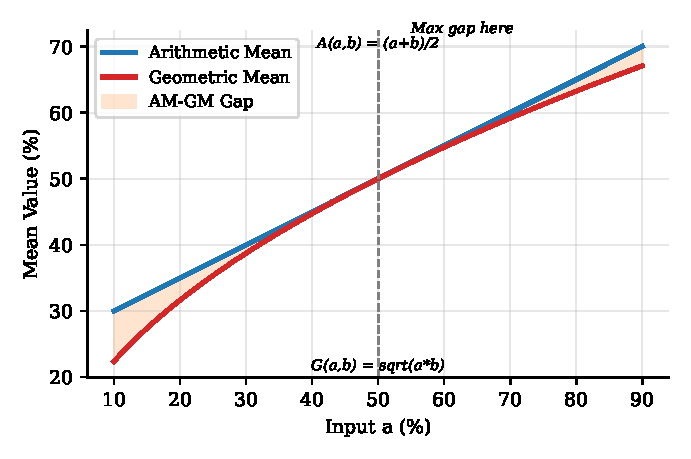
\includegraphics[width=0.8\textwidth]{figures/fig_geometric_vs_arithmetic_mean.pdf}
    \caption{Geometric vs.\ arithmetic mean: the geometric mean penalises disagreement between inputs.}
    \label{fig:geometric-vs-arithmetic-mean}
\end{figure}

The geometric mean is preferred over the arithmetic mean for combining classifier confidences because it penalises disagreement: if either score is low, their product drops sharply, producing a low combined confidence. This property naturally routes uncertain cases toward manual review, where a single high-confidence source should not dominate the decision.

\subsection{Agreement and Disagreement Detection}
\label{sec:agreement-detection}

Agreement detection determines whether two or more decision sources produce the same predicted class, and adjusts the combination strategy accordingly. The agreement indicator between two sources $s_1$ and $s_2$ is:

\begin{equation}
\text{agree}(s_1, s_2) = \mathbb{I}\left(\arg\max s_1 = \arg\max s_2\right)
\label{eq:agreement}
\end{equation}

When sources disagree, the confidence gap quantifies the magnitude of disagreement:

\begin{equation}
\Delta = |c_{\text{rule}} - c_{\text{ml}}|
\label{eq:confidence-gap}
\end{equation}

A tolerance threshold determines whether the disagreement is within acceptable bounds:

\begin{equation}
\text{tolerate}(\Delta) = \begin{cases} \text{true} & \text{if } \Delta \leq \tau_{\text{gap}} \\ \text{false} & \text{otherwise} \end{cases}
\label{eq:disagreement-tolerance}
\end{equation}

Agreement detection enables adaptive fusion: when sources agree on the predicted class, the combined confidence receives an agreement bonus and higher effective weights; when they disagree, the combination shifts toward a more conservative decision, potentially routing to manual review.

\subsection{Confidence Clamping and Bounding}
\label{sec:confidence-clamping}

Clamping constrains a computed confidence score to a valid range $[c_{\min}, c_{\max}]$ to prevent overflow, underflow, or unrealistic extreme values:

\begin{equation}
\text{clamp}(c, c_{\min}, c_{\max}) = \min(c_{\max}, \max(c_{\min}, c))
\label{eq:clamp}
\end{equation}

In practice, the final confidence is computed as:

\begin{equation}
c_{\text{final}} = \text{round}(\text{clamp}(c_{\text{raw}}, 0.0, 98.0), 1)
\label{eq:final-confidence}
\end{equation}

The upper bound of 98.0 (rather than 100.0) reflects inherent model uncertainty: no statistical model should claim 100\% confidence, as there is always a probability of error. The rounding to one decimal place provides a clean user-facing output while avoiding false precision from floating-point arithmetic.

Clamping ensures numerical stability and prevents edge-case scores from triggering incorrect downstream decisions. Combined with the three-tier thresholding described in Section~\ref{sec:confidence-thresholding}, it creates a decision system that is both robust to extreme inputs and transparent in its routing logic.

% ============================================================
\section{Large Language Models}
\label{sec:llms}

Large Language Models (LLMs) are neural networks trained on massive text corpora to understand and generate human language. This section covers the transformer architecture underlying modern LLMs, prompt engineering techniques, inference strategies, and practical integration patterns.

\subsection{Transformer Architecture}
\label{sec:transformer}

The Transformer is a neural network architecture that processes sequences using self-attention mechanisms, allowing every token in a sequence to attend to every other token simultaneously without recurrence. Introduced by Vaswani et al.\ (2017), it forms the backbone of all modern LLMs.

The core computation in a Transformer encoder layer is scaled dot-product attention:

\begin{equation}
\text{Attention}(Q, K, V) = \text{softmax}\left(\frac{QK^T}{\sqrt{d_k}}\right)V
\label{eq:attention}
\end{equation}

where $Q$ (queries), $K$ (keys), and $V$ (values) are linear projections of the input, and $d_k$ is the key dimension. The scaling factor $\sqrt{d_k}$ prevents dot products from growing too large, which would push the softmax into regions with vanishing gradients.

Multi-head attention extends this by running $h$ parallel attention operations with different learned projections:

\begin{align}
\text{MultiHead}(Q, K, V) &= \text{Concat}(\text{head}_1, \ldots, \text{head}_h)W^O \label{eq:multihead-1} \\
\text{head}_i &= \text{Attention}(QW_i^Q, KW_i^K, VW_i^V) \label{eq:multihead-2}
\end{align}

Positional information is injected through sinusoidal encodings:

\begin{align}
PE_{(pos, 2i)} &= \sin\left(\frac{pos}{10000^{2i/d_{\text{model}}}}\right) \label{eq:positional-1} \\
PE_{(pos, 2i+1)} &= \cos\left(\frac{pos}{10000^{2i/d_{\text{model}}}}\right) \label{eq:positional-2}
\end{align}

\begin{figure}[H]
    \centering
    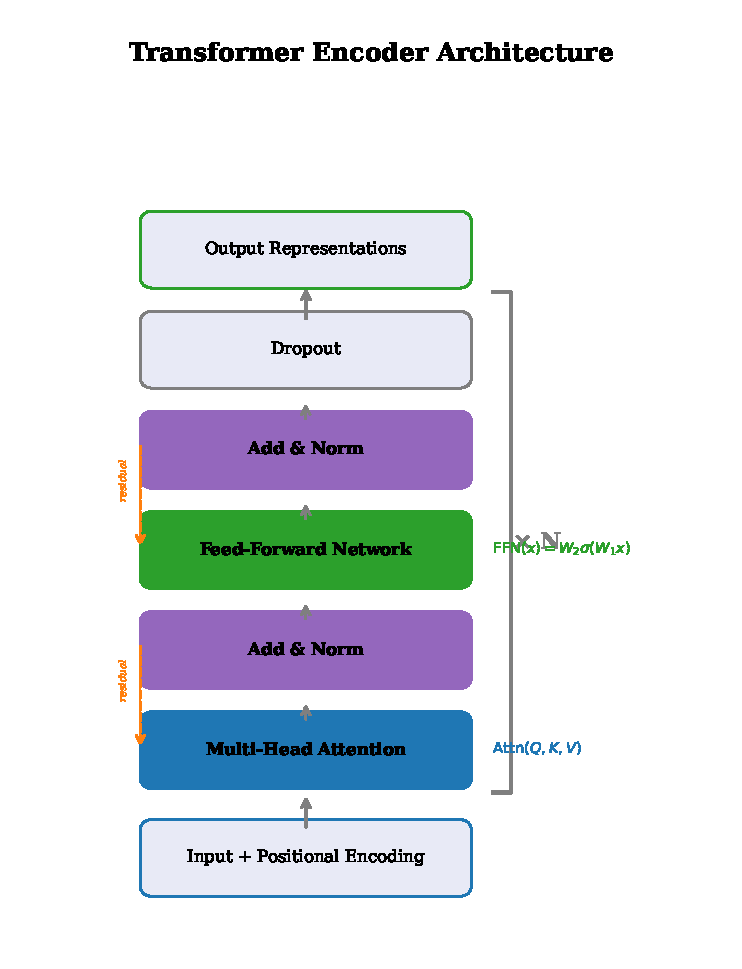
\includegraphics[width=0.85\textwidth]{figures/fig_transformer_architecture.pdf}
    \caption{Transformer architecture: scaled dot-product attention with multi-head mechanism.}
    \label{fig:transformer-architecture}
\end{figure}

The self-attention mechanism enables the model to resolve semantic ambiguities by attending to contextual cues across the entire input sequence, a capability that simple keyword matching cannot replicate. Understanding the underlying architecture is relevant because it motivates the design choices in prompt engineering (Section~\ref{sec:prompt-engineering}) and explains why LLMs can interpret free-text inputs with nuance.

\subsection{Prompt Engineering}
\label{sec:prompt-engineering}

Prompt engineering is the practice of designing the natural-language input (prompt) to an LLM to elicit a desired format, style, or content in its response. Because LLMs are trained to complete text, the phrasing, structure, and constraints embedded in the prompt strongly influence the output.

Four key design patterns form the foundation of effective prompt engineering:

\begin{enumerate}
    \item \textbf{Role framing:} Assigning a persona (e.g., ``You are an expert automotive warranty analyst'') grounds the model's responses in the relevant domain vocabulary and reasoning style.
    \item \textbf{Explicit output format specification:} Instructing the model to respond only with JSON in an exact schema eliminates formatting variability and enables programmatic parsing.
    \item \textbf{Enumerated constraints:} Listing allowed values for categorical outputs (e.g., ``category must be one of: moisture\_damage, physical\_damage, ntf, electrical\_issue, engine\_symptom, communication\_fault, other'') eliminates hallucinated categories.
    \item \textbf{Disambiguation rules:} Providing ordered priority rules for ambiguous cases (e.g., ``overheating maps to engine\_symptom, not electrical\_issue'') ensures deterministic categorisation.
\end{enumerate}

\begin{figure}[H]
    \centering
    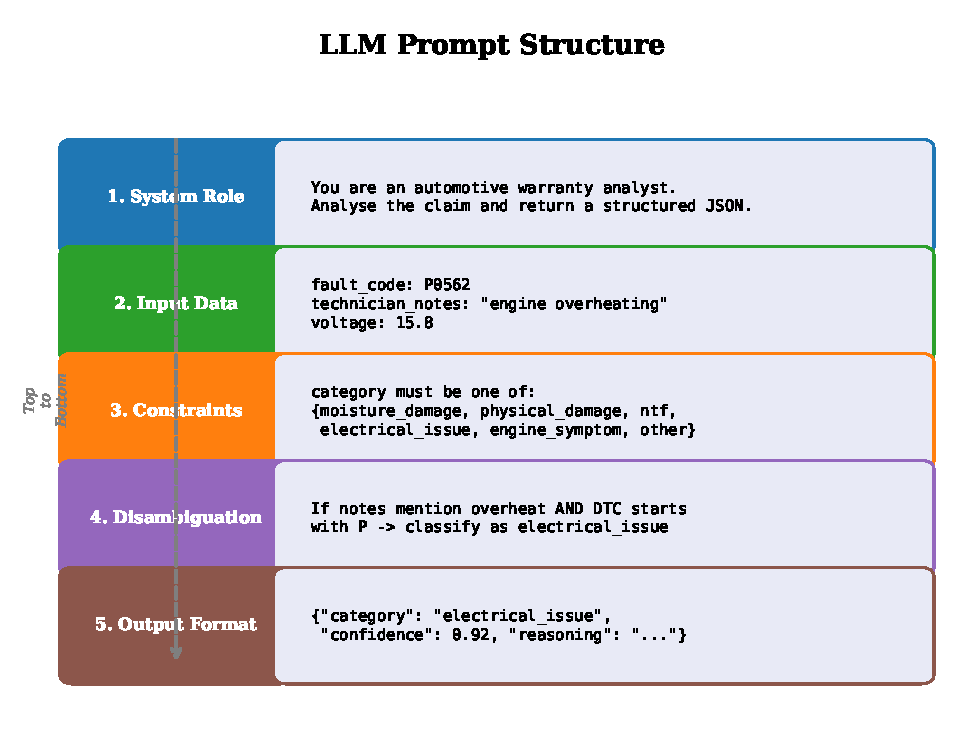
\includegraphics[width=0.85\textwidth]{figures/fig_prompt_structure.pdf}
    \caption{Structured prompt anatomy: role framing, output constraints, enumerated options, and disambiguation rules.}
    \label{fig:prompt-structure}
\end{figure}

\subsection{Zero-Shot Inference}
\label{sec:zero-shot}

Zero-shot inference refers to using a pre-trained LLM to perform a task it was not explicitly fine-tuned for, relying solely on the instruction provided in the prompt without any labelled examples. The model's predicted probability for class $c$ given instruction $I$ and input $x$ is:

\begin{equation}
P(c \mid I, x) = \frac{\exp(s(c, I, x))}{\sum_{c' \in \mathcal{C}} \exp(s(c', I, x))}
\label{eq:zero-shot}
\end{equation}

where $s(\cdot)$ is the model's scoring function and $\mathcal{C}$ is the set of allowed categories.

Zero-shot inference enables rapid task adaptation without collecting labelled training data. The trade-off is lower accuracy compared to fine-tuned models, since the model relies entirely on its pre-trained knowledge and the prompt's instructions. When the prompt constraints are sufficiently tight (enumerated categories, JSON format, disambiguation rules), zero-shot performance can approach that of fine-tuned approaches for classification tasks.

\subsection{Temperature and Seeded Generation}
\label{sec:temperature}

Temperature controls the randomness of token sampling in autoregressive language models. The probability of selecting token $x_i$ given context $x_{<i}$ is scaled by temperature $T$:

\begin{equation}
P(x_i \mid x_{<i}) = \frac{\exp(z_i / T)}{\sum_j \exp(z_j / T)}
\label{eq:temperature}
\end{equation}

where $z_i$ are the logits (unnormalised scores) produced by the model. In the limiting cases:

\begin{equation}
\lim_{T \to 0} P(x_i) = \begin{cases} 1 & \text{if } i = \arg\max_j z_j \\ 0 & \text{otherwise} \end{cases}
\label{eq:temp-zero}
\end{equation}

\begin{equation}
\lim_{T \to \infty} P(x_i) = \frac{1}{|\mathcal{V}|}
\label{eq:temp-infinity}
\end{equation}

where $\mathcal{V}$ is the vocabulary size. At $T = 0$ (greedy decoding), the model always selects the highest-probability token, producing deterministic outputs. At high temperatures, the distribution flattens, introducing more randomness.

\begin{figure}[H]
    \centering
    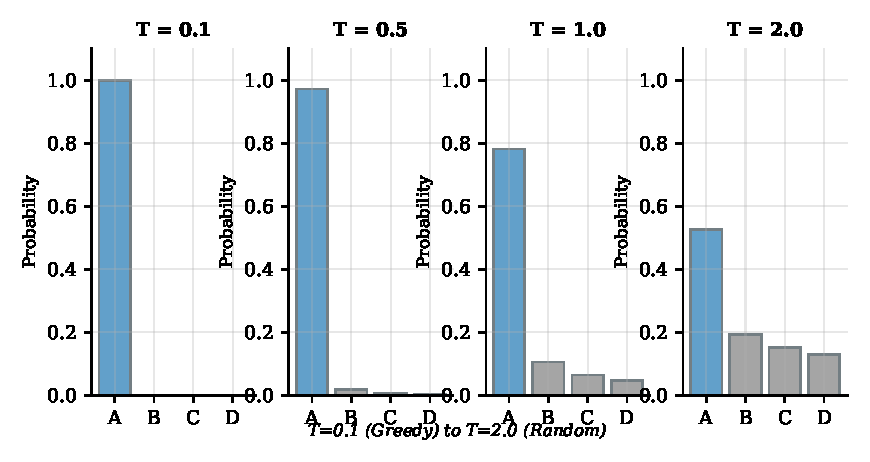
\includegraphics[width=0.85\textwidth]{figures/fig_temperature_effect.pdf}
    \caption{Temperature effect on output distribution: low temperature sharpens, high temperature flattens.}
    \label{fig:temperature-effect}
\end{figure}

Setting $T = 0$ with a fixed random seed produces completely deterministic outputs, which is essential for reproducible classification pipelines where the same input must always yield the same classification. Higher temperatures may be used for creative generation tasks where output diversity is desired.

\subsection{JSON-Constrained Output Generation}
\label{sec:json-constrained}

Constraining LLM outputs to valid JSON format bridges the gap between free-text generation and structured data processing. Two mechanisms enforce JSON compliance:

\begin{enumerate}
    \item \textbf{Prompt-level constraints:} Explicit instructions in the prompt (e.g., ``Respond only with valid JSON containing the keys: category, confidence, reason'') guide the model toward structured output.
    \item \textbf{API-level format enforcement:} Modern LLM APIs accept a \texttt{response\_format} parameter (e.g., \texttt{\{"type": "json\_object"\}}) that instructs the model to produce syntactically valid JSON by constraining the token generation process at the decoding level.
\end{enumerate}

Both mechanisms should be used together for maximum reliability. When the JSON response cannot be parsed (due to formatting errors or schema violations), a default value fallback strategy provides safe degradation: each expected key is assigned a sensible default (e.g., \texttt{"confidence": 0.0}, \texttt{"category": "other"}) so that the pipeline can continue operating even with malformed LLM output.

\subsection{API-Based LLM Integration}
\label{sec:api-llm}

Accessing LLM capabilities through HTTP-based API endpoints decouples application logic from model infrastructure. The standard interface is the chat completions endpoint:

\begin{equation}
\text{POST } /v1/chat/completions
\label{eq:api-endpoint}
\end{equation}

with a JSON request body specifying the model, messages, and parameters:

\begin{equation}
\text{Body: } \{\texttt{"model"}: m, \texttt{"messages"}: [\{\texttt{"role"}: \texttt{"user"}, \texttt{"content"}: p\}], \texttt{"temperature"}: T\}
\label{eq:api-body}
\end{equation}

\begin{figure}[H]
    \centering
    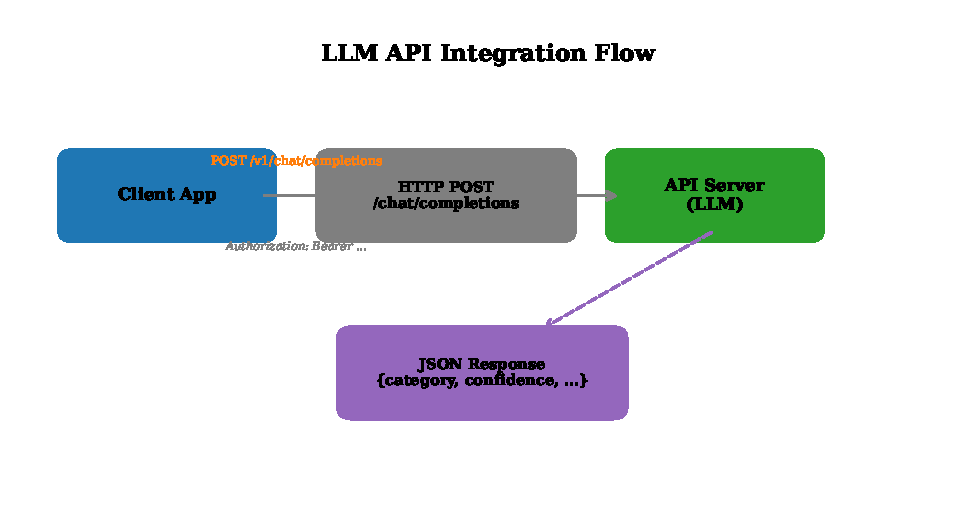
\includegraphics[width=0.85\textwidth]{figures/fig_api_integration_flow.pdf}
    \caption{API-based LLM integration: request, inference, and response cycle.}
    \label{fig:api-integration-flow}
\end{figure}

A provider-agnostic interface abstracts over different API services (e.g., OpenAI, OpenRouter), selecting the primary provider when available and falling back to a secondary provider when the primary is unavailable. This pattern enables switching between providers without changes to the application logic.

\subsection{Retry with Exponential Backoff}
\label{sec:exponential-backoff}

Exponential backoff is a fault-tolerance strategy that retries failed API calls with exponentially increasing delays between attempts. The delay before attempt $k$ (0-indexed) is:

\begin{equation}
\text{delay}_k = \text{base\_delay} \times 2^k
\label{eq:backoff-delay}
\end{equation}

The total wait time for $n$ retries is:

\begin{equation}
T_{\text{total}} = \sum_{k=0}^{n-1} \text{base\_delay} \times 2^k = \text{base\_delay} \times (2^n - 1)
\label{eq:backoff-total}
\end{equation}

\begin{figure}[H]
    \centering
    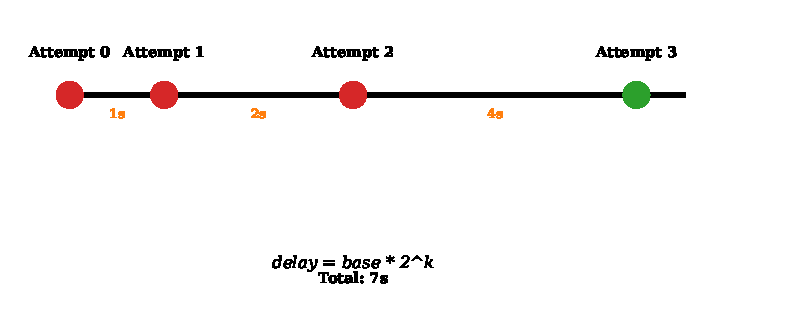
\includegraphics[width=0.85\textwidth]{figures/fig_exponential_backoff.pdf}
    \caption{Exponential backoff: retry attempts with increasing delays between calls.}
    \label{fig:exponential-backoff}
\end{figure}

Exponential backoff handles transient network failures and rate limiting (HTTP 429 responses) without overwhelming the API server. Common configuration includes a maximum of 2--3 retries with a base delay of 1--2 seconds, giving a total worst-case wait of 3--7 seconds.

\subsection{Graceful Degradation and Fallback Chains}
\label{sec:graceful-degradation}

Graceful degradation is a system design pattern where the application continues to operate at reduced functionality when a component fails, by switching to alternative implementations. A fallback chain defines an ordered sequence of implementations, from most capable to least:

\begin{equation}
\text{output}(x) = \begin{cases}
f_{\text{primary}}(x) & \text{if } f_{\text{primary}} \text{ succeeds} \\
f_{\text{fallback}_1}(x) & \text{if } f_{\text{primary}} \text{ fails, } f_{\text{fallback}_1} \text{ succeeds} \\
\vdots & \\
f_{\text{default}}(x) & \text{otherwise}
\end{cases}
\label{eq:fallback-chain}
\end{equation}

\begin{figure}[H]
    \centering
    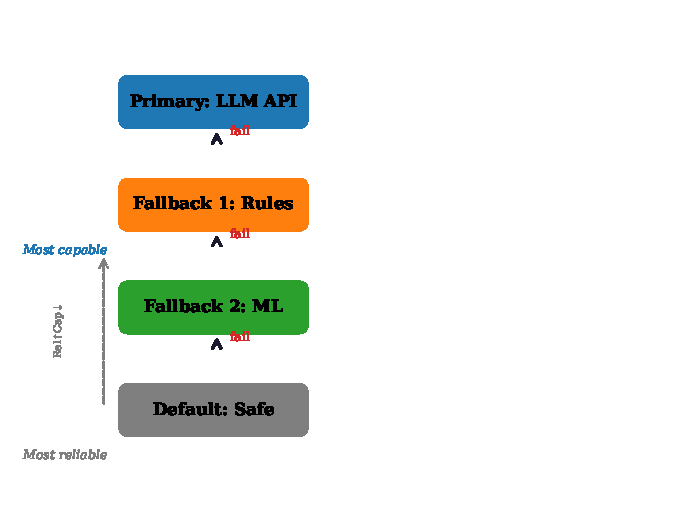
\includegraphics[width=0.85\textwidth]{figures/fig_fallback_chain.pdf}
    \caption{Fallback chain: preferred implementation $\rightarrow$ alternative $\rightarrow$ default.}
    \label{fig:fallback-chain}
\end{figure}

In a multi-stage pipeline, each stage implements its own fallback chain independently. This ensures that the failure of a single component (e.g., LLM API unavailability) does not cascade to disable the entire system. The trade-off is reduced capability in degraded mode; for example, losing LLM semantic understanding but retaining rule-based and ML-based decisions.

% ============================================================
\section{Model Evaluation Metrics}
\label{sec:evaluation-metrics}

Evaluation metrics quantify the performance of machine learning models, enabling comparison between algorithms, hyperparameter configurations, and system architectures. This section defines the metrics used throughout classification system evaluation.

\subsection{Accuracy}
\label{sec:accuracy}

Accuracy is the proportion of correct predictions among all predictions made:

\begin{equation}
\text{Accuracy} = \frac{TP + TN}{TP + TN + FP + FN} = \frac{\text{correct predictions}}{\text{total predictions}}
\label{eq:accuracy}
\end{equation}

While intuitive, accuracy can be misleading on imbalanced datasets where one class dominates. A classifier that always predicts the majority class can achieve high accuracy without learning any meaningful patterns.

\subsection{Precision}
\label{sec:precision}

Precision measures the proportion of positive predictions that are actually correct for a given class:

\begin{equation}
\text{Precision}(c) = \frac{TP_c}{TP_c + FP_c}
\label{eq:precision}
\end{equation}

where $TP_c$ is the number of true positives for class $c$ and $FP_c$ is the number of false positives (instances incorrectly predicted as class $c$).

For multi-class evaluation, two averaging strategies are common:

\begin{itemize}
    \item \textbf{Macro precision:} Unweighted average over all classes:
    \begin{equation}
    \text{Precision}_{\text{macro}} = \frac{1}{K} \sum_{c=1}^{K} \text{Precision}(c)
    \label{eq:precision-macro}
    \end{equation}
    \item \textbf{Weighted precision:} Average weighted by class frequency:
    \begin{equation}
    \text{Precision}_{\text{weighted}} = \sum_{c=1}^{K} \frac{N_c}{N} \cdot \text{Precision}(c)
    \label{eq:precision-weighted}
    \end{equation}
\end{itemize}

Precision is critical when false positives are costly. In a warranty analysis context, high precision for ``Customer Failure'' means that when the system claims a failure is customer-induced, it is usually correct.

\subsection{Recall (Sensitivity)}
\label{sec:recall}

Recall (also called sensitivity or true positive rate) measures the proportion of actual positives that are correctly identified:

\begin{equation}
\text{Recall}(c) = \frac{TP_c}{TP_c + FN_c}
\label{eq:recall}
\end{equation}

where $FN_c$ is the number of false negatives for class $c$ (instances of class $c$ incorrectly predicted as a different class).

Macro and weighted averaging follow the same pattern as precision (Equations~\ref{eq:precision-macro} and~\ref{eq:precision-weighted}).

Recall is critical when false negatives are costly. In a warranty analysis context, high recall for ``Production Failure'' means that the system correctly identifies the vast majority of genuine production defects, minimising the risk of incorrectly rejecting valid warranty claims.

\subsection{F1 Score}
\label{sec:f1-score}

The F1 score is the harmonic mean of precision and recall, providing a single metric that balances both concerns:

\begin{equation}
F1(c) = \frac{2 \cdot \text{Precision}(c) \cdot \text{Recall}(c)}{\text{Precision}(c) + \text{Recall}(c)} = \frac{2TP_c}{2TP_c + FP_c + FN_c}
\label{eq:f1}
\end{equation}

The harmonic mean penalises extreme imbalance between precision and recall more severely than the arithmetic mean: a high F1 requires both precision and recall to be reasonably high.

Macro and weighted averaging follow the same pattern:

\begin{align}
F1_{\text{macro}} &= \frac{1}{K} \sum_{c=1}^{K} F1(c) \label{eq:f1-macro} \\
F1_{\text{weighted}} &= \sum_{c=1}^{K} \frac{N_c}{N} \cdot F1(c) \label{eq:f1-weighted}
\end{align}

\begin{figure}[H]
    \centering
    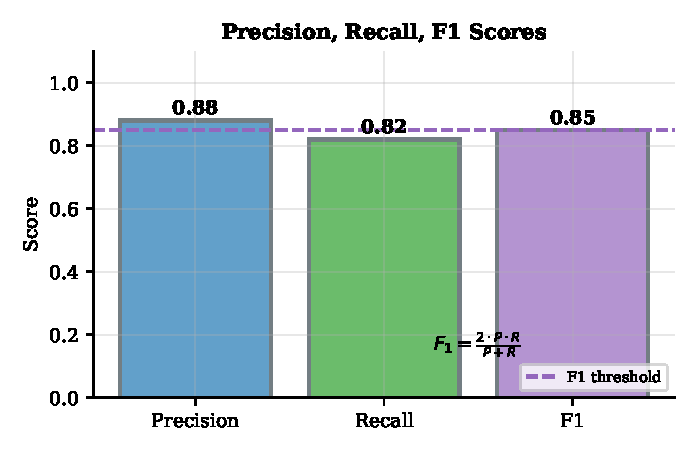
\includegraphics[width=0.8\textwidth]{figures/fig_precision_recall_f1.pdf}
    \caption{Precision, recall, and F1: relationships and trade-offs.}
    \label{fig:precision-recall-f1}
\end{figure}

\subsection{Confusion Matrix}
\label{sec:confusion-matrix}

A confusion matrix is a $K \times K$ table where entry $(i, j)$ counts the number of instances whose true class is $i$ and predicted class is $j$:

\begin{equation}
C_{ij} = \sum_{n=1}^{N} \mathbb{I}(y^{(n)} = c_i \land \hat{y}^{(n)} = c_j)
\label{eq:confusion-matrix}
\end{equation}

Row sums give the actual class counts ($TP_c + FN_c$ for class $c$), and column sums give the predicted class counts ($TP_c + FP_c$ for class $c$).

\begin{figure}[H]
    \centering
    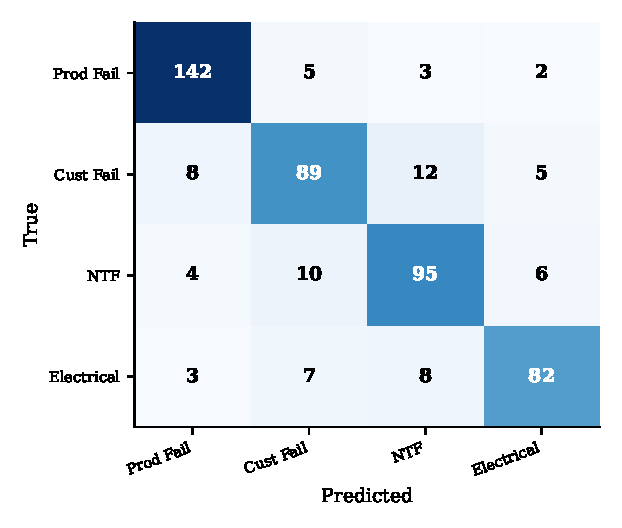
\includegraphics[width=0.8\textwidth]{figures/fig_confusion_matrix.pdf}
    \caption{Confusion matrix: true labels (rows) vs.\ predicted labels (columns).}
    \label{fig:confusion-matrix}
\end{figure}

The confusion matrix reveals which classes are confused with each other, guiding targeted model improvements. Off-diagonal entries indicate systematic misclassifications that may be addressable through additional features, more training data, or rule-based corrections.

\subsection{Classification Report}
\label{sec:classification-report}

A classification report tabulates precision, recall, F1 score, and support (number of true instances) for each class, along with macro and weighted averages. It provides a per-class performance breakdown in a single view, making it easy to identify which classes are well-classified and which require attention.

\begin{table}[H]
\centering
\caption{Example classification report structure.}
\label{tab:classification-report}
\begin{tabular}{lcccc}
\toprule
\textbf{Class} & \textbf{Precision} & \textbf{Recall} & \textbf{F1-Score} & \textbf{Support} \\
\midrule
Class A & 0.92 & 0.88 & 0.90 & 150 \\
Class B & 0.78 & 0.85 & 0.81 & 200 \\
Class C & 0.95 & 0.91 & 0.93 & 100 \\
\midrule
Macro Avg & 0.88 & 0.88 & 0.88 & 450 \\
Weighted Avg & 0.87 & 0.87 & 0.87 & 450 \\
\bottomrule
\end{tabular}
\end{table}

\subsection{Feature Importance (Gini Importance)}
\label{sec:feature-importance}

Feature importance quantifies the contribution of each input feature to the model's predictions, computed as the total reduction in impurity attributable to splits on that feature, averaged across all trees in an ensemble.

For a single tree $t$, the importance of feature $j$ is:

\begin{equation}
\text{Imp}_j^{(t)} = \sum_{s \in \text{splits on } j} N_s \cdot \Delta G_s
\label{eq:feature-importance-tree}
\end{equation}

where $N_s$ is the number of samples at split $s$ and $\Delta G_s$ is the impurity reduction at that split. For an ensemble of $T$ trees:

\begin{equation}
\text{Imp}_j = \frac{1}{T} \sum_{t=1}^{T} \text{Imp}_j^{(t)}
\label{eq:feature-importance-ensemble}
\end{equation}

Normalised importance scales each feature's importance relative to the total:

\begin{equation}
\text{Imp}_j^{\text{norm}} = \frac{\text{Imp}_j}{\sum_{k=1}^{p} \text{Imp}_k}
\label{eq:feature-importance-normalised}
\end{equation}

\begin{figure}[H]
    \centering
    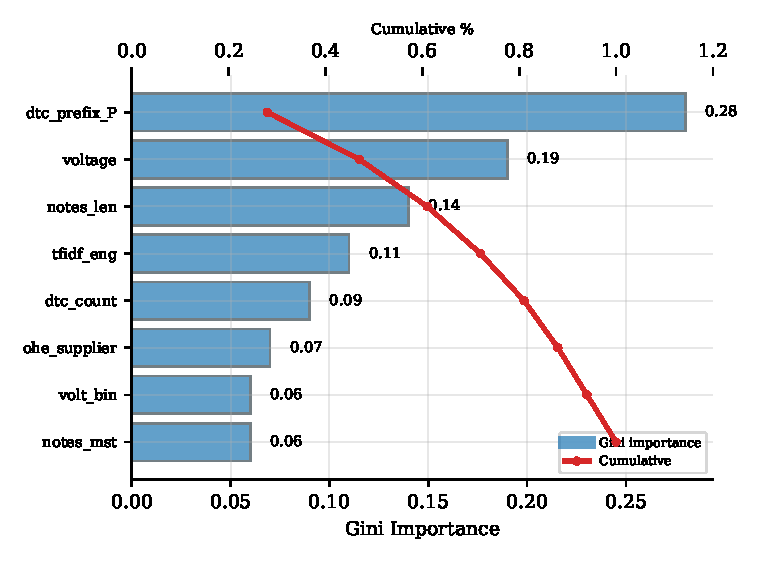
\includegraphics[width=0.8\textwidth]{figures/fig_feature_importance.pdf}
    \caption{Feature importance: horizontal bar chart ranking features by their contribution.}
    \label{fig:feature-importance}
\end{figure}

Feature importance enables model interpretability and feature selection. In gradient-boosted models, features with high importance are those that the model uses most frequently and effectively for splitting decisions.

\subsection{Calibration Curves}
\label{sec:calibration}

A calibration curve (reliability diagram) compares predicted probabilities against actual observed frequencies. For a perfectly calibrated model, the predicted probability equals the observed frequency:

\begin{equation}
P(\hat{y} = y \mid \hat{p} = p) = p \quad \forall p \in [0, 1]
\label{eq:perfect-calibration}
\end{equation}

The expected calibration error (ECE) quantifies the average gap between predicted confidence and observed accuracy:

\begin{equation}
\text{ECE} = \sum_{m=1}^{M} \frac{|B_m|}{N} | \text{acc}(B_m) - \text{conf}(B_m) |
\label{eq:ece}
\end{equation}

where $B_m$ is the $m$-th probability bin, $\text{acc}(B_m)$ is the fraction of correct predictions in the bin, and $\text{conf}(B_m)$ is the mean predicted confidence.

\begin{figure}[H]
    \centering
    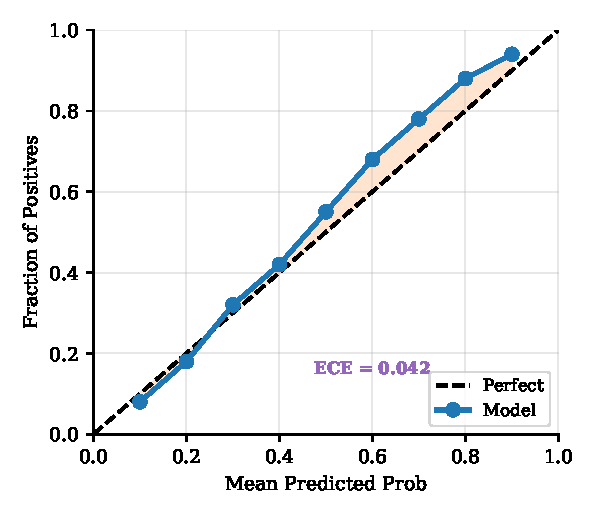
\includegraphics[width=0.8\textwidth]{figures/fig_calibration_curve.pdf}
    \caption{Calibration curve: predicted probability vs.\ observed frequency.}
    \label{fig:calibration-curve}
\end{figure}

Calibration is essential for cascade architectures where one classifier's probabilities become another's input features. Poorly calibrated probabilities (overconfident near 0/1 or underconfident near 0.5) degrade downstream classifier performance because the second-stage model receives unreliable signal from the first stage.

% ============================================================
\section{Synthetic Data Generation}
\label{sec:synthetic-data}

Synthetic data generation creates realistic artificial datasets that mimic the statistical properties of real-world data. This section covers the probability distributions, sampling strategies, and noise injection techniques used to produce training data that captures the complexity and imperfections of genuine datasets.

\subsection{Probability Distributions}
\label{sec:probability-distributions}

Probability distributions model the likelihood of different outcomes for a random variable. Three distributions are particularly important for generating realistic synthetic features:

\textbf{Normal (Gaussian) distribution} produces symmetric, bell-shaped values centred on the mean $\mu$ with spread $\sigma$:

\begin{equation}
f(x \mid \mu, \sigma^2) = \frac{1}{\sqrt{2\pi\sigma^2}} \exp\left(-\frac{(x-\mu)^2}{2\sigma^2}\right)
\label{eq:normal}
\end{equation}

\textbf{Truncated normal distribution} restricts sampling to a bounded interval $[a, b]$, preventing values outside realistic ranges:

\begin{equation}
f_T(x) = \frac{\phi\left(\frac{x-\mu}{\sigma}\right)}{\sigma\left[\Phi\left(\frac{b-\mu}{\sigma}\right) - \Phi\left(\frac{a-\mu}{\sigma}\right)\right]} \quad \text{for } x \in [a, b]
\label{eq:truncated-normal}
\end{equation}

where $\phi$ is the standard normal PDF and $\Phi$ is the standard normal CDF. The truncated normal is used when the underlying process is approximately normal but physical constraints impose hard bounds (e.g., voltage cannot be negative).

\textbf{Log-normal distribution} produces right-skewed positive values, appropriate for variables that grow multiplicatively:

\begin{equation}
f(x \mid \mu, \sigma) = \frac{1}{x\sigma\sqrt{2\pi}} \exp\left(-\frac{(\ln x - \mu)^2}{2\sigma^2}\right) \quad \text{for } x > 0
\label{eq:lognormal}
\end{equation}

\begin{figure}[H]
    \centering
    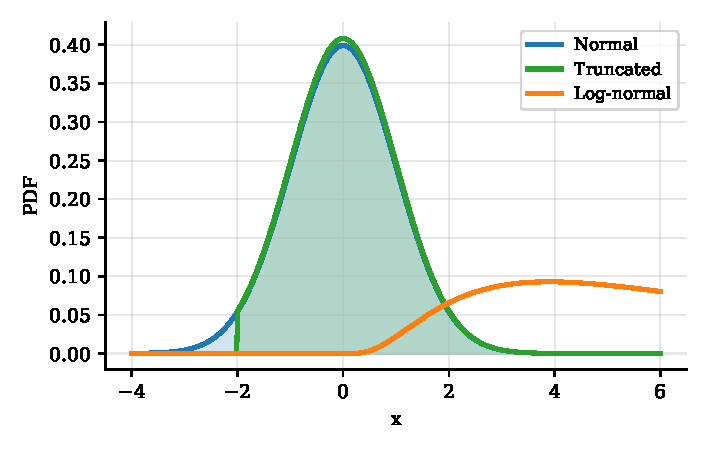
\includegraphics[width=0.85\textwidth]{figures/fig_distributions.pdf}
    \caption{Probability distributions: normal, truncated normal, and log-normal.}
    \label{fig:distributions}
\end{figure}

\subsection{Weighted Random Sampling}
\label{sec:weighted-sampling}

Weighted random sampling draws from a discrete distribution where each element has an assigned probability:

\begin{equation}
P(X = i) = w_i, \quad \text{where } \sum_{i=1}^{K} w_i = 1
\label{eq:weighted-sampling}
\end{equation}

Inverse transform sampling converts a uniform random variable $U \sim \text{Uniform}(0, 1)$ to the desired distribution:

\begin{equation}
X = F^{-1}(U)
\label{eq:inverse-transform}
\end{equation}

where $F$ is the cumulative distribution function. Weighted sampling controls class balance in synthetic datasets, enabling modelling of realistic class prevalence where some categories occur far more frequently than others.

\begin{figure}[H]
    \centering
    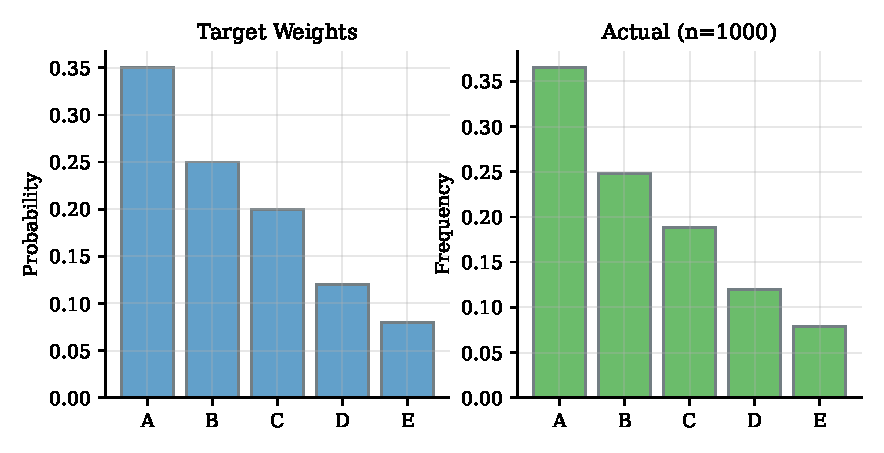
\includegraphics[width=0.8\textwidth]{figures/fig_weighted_sampling.pdf}
    \caption{Weighted random sampling: category weights determine sample frequencies.}
    \label{fig:weighted-sampling}
\end{figure}

\subsection{Bimodal and Mixture Distributions}
\label{sec:mixture-distributions}

A mixture distribution combines two or more component distributions, each with its own parameters and mixing weight:

\begin{equation}
f(x) = \sum_{k=1}^{K} \pi_k \cdot f_k(x \mid \theta_k)
\label{eq:mixture}
\end{equation}

where $\pi_k > 0$ are mixing weights with $\sum_k \pi_k = 1$, and $f_k$ are component densities with parameters $\theta_k$. A two-component Gaussian mixture is:

\begin{equation}
f(x) = \pi_1 \cdot \mathcal{N}(x \mid \mu_1, \sigma_1^2) + \pi_2 \cdot \mathcal{N}(x \mid \mu_2, \sigma_2^2)
\label{eq:bimodal}
\end{equation}

\begin{figure}[H]
    \centering
    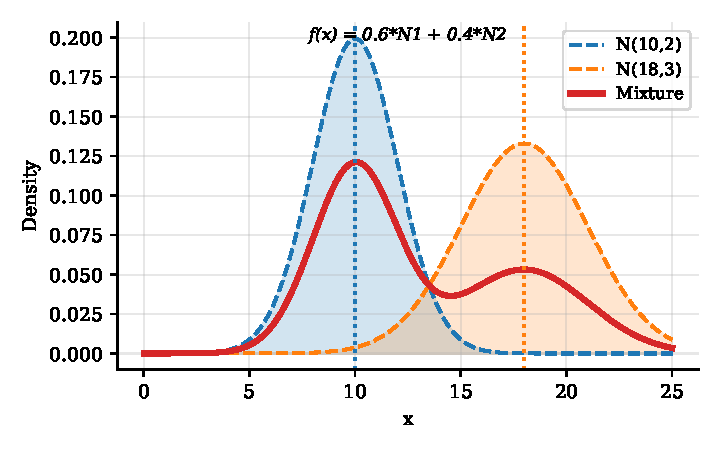
\includegraphics[width=0.8\textwidth]{figures/fig_mixture_distribution.pdf}
    \caption{Bimodal mixture distribution: two Gaussian components with mixing weights $\pi_1$ and $\pi_2$.}
    \label{fig:mixture-distribution}
\end{figure}

Mixture distributions model features with multiple modes, such as voltage readings that cluster around both normal and abnormal operating ranges, or mileage distributions with distinct early-life and wear-and-tear subpopulations.

\subsection{Correlated Feature Generation}
\label{sec:correlated-features}

Real-world features often exhibit statistical dependence. A bivariate normal distribution with correlation $\rho$ generates pairs of correlated features:

\begin{equation}
\begin{pmatrix} X_1 \\ X_2 \end{pmatrix} \sim \mathcal{N}\left(\begin{pmatrix} \mu_1 \\ \mu_2 \end{pmatrix}, \begin{pmatrix} \sigma_1^2 & \rho\sigma_1\sigma_2 \\ \rho\sigma_1\sigma_2 & \sigma_2^2 \end{pmatrix}\right)
\label{eq:bivariate-normal}
\end{equation}

Correlated samples are generated via Cholesky decomposition of the covariance matrix:

\begin{equation}
X = \mu + L Z, \quad Z \sim \mathcal{N}(0, I)
\label{eq:cholesky}
\end{equation}

where $\Sigma = LL^T$ is the Cholesky decomposition and $Z$ is a vector of independent standard normals.

\begin{figure}[H]
    \centering
    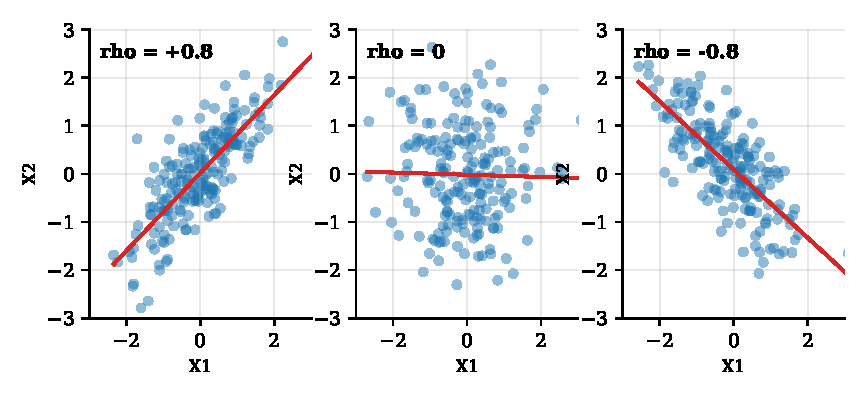
\includegraphics[width=0.8\textwidth]{figures/fig_correlated_features.pdf}
    \caption{Correlated feature generation: positive ($\rho = 0.8$), zero ($\rho = 0$), and negative ($\rho = -0.8$) correlations.}
    \label{fig:correlated-features}
\end{figure}

Generating correlated features ensures synthetic data reflects realistic feature relationships (e.g., higher mileage correlating with older vehicle age), preventing models from learning spurious patterns that would not exist in production data.

\subsection{Label Noise Injection}
\label{sec:label-noise}

Label noise injection intentionally flips a fraction of labels to simulate annotation errors, ambiguous cases, or inherent uncertainty. Symmetric noise flips a label to any other class with equal probability:

\begin{equation}
\tilde{y}_i = \begin{cases} y_i & \text{with probability } 1 - \eta \\ \text{Uniform}(\mathcal{C} \setminus \{y_i\}) & \text{with probability } \eta \end{cases}
\label{eq:symmetric-noise}
\end{equation}

Asymmetric noise flips to a specific confusing class, simulating realistic mislabelling patterns:

\begin{equation}
\tilde{y}_i = \begin{cases} y_i & \text{with probability } 1 - \eta \\ c_{\text{confusing}} & \text{with probability } \eta \end{cases}
\label{eq:asymmetric-noise}
\end{equation}

Label noise produces realistic datasets where patterns hold approximately but not perfectly, testing model robustness to annotation uncertainty. A model trained on perfectly clean data may achieve unrealistically high accuracy that does not generalise to noisy real-world inputs.

\subsection{Temporal Drift Modelling}
\label{sec:temporal-drift}

Temporal drift simulates changes in data distribution over time, reflecting evolving failure modes, changing usage patterns, or updated designs. Linear drift shifts the mean of a distribution over time:

\begin{equation}
\mu(t) = \mu_0 + \delta \cdot t
\label{eq:linear-drift}
\end{equation}

where $\mu_0$ is the initial mean and $\delta$ is the drift rate per time unit. Time-weighted sampling controls the relative frequency of samples from different time periods:

\begin{equation}
P(\text{sample from period } t) \propto w_t
\label{eq:time-weights}
\end{equation}

Temporal drift ensures synthetic datasets capture the evolution of patterns across time, such as increasing electrical failure rates in newer vehicle models or decreasing mechanical failure rates after a design improvement.

\subsection{Seeded Random Number Generation}
\label{sec:seeded-rng}

Pseudo-random number generators (PRNGs) produce deterministic sequences of numbers that appear random but are fully determined by an initial seed value $X_0$. The linear congruential generator is a simple example:

\begin{equation}
X_{n+1} = (aX_n + c) \mod m
\label{eq:lcg}
\end{equation}

where $a$ is the multiplier, $c$ is the increment, and $m$ is the modulus. Modern PRNGs (such as the Mersenne Twister) use more sophisticated algorithms but follow the same seed-determinism principle.

Setting a fixed seed before data generation ensures that the same sequence of ``random'' choices is produced on every run, making the synthetic dataset reproducible. This is critical for experimental reproducibility: the same seed produces identical datasets, train/test splits, and model initialisations across different machines and runs.

% ============================================================
\section{System Architecture Patterns}
\label{sec:architecture-patterns}

This section covers software architecture patterns that enable reliable, maintainable, and scalable ML system deployment.

\subsection{Multi-Stage Pipeline Architecture}
\label{sec:pipeline-architecture}

A multi-stage pipeline processes data through a sequence of stages, where each stage performs a specific transformation and the output of one stage serves as input to the next:

\begin{equation}
y = f_n(f_{n-1}(\cdots f_2(f_1(x))\cdots))
\label{eq:pipeline-composition}
\end{equation}

\begin{figure}[H]
    \centering
    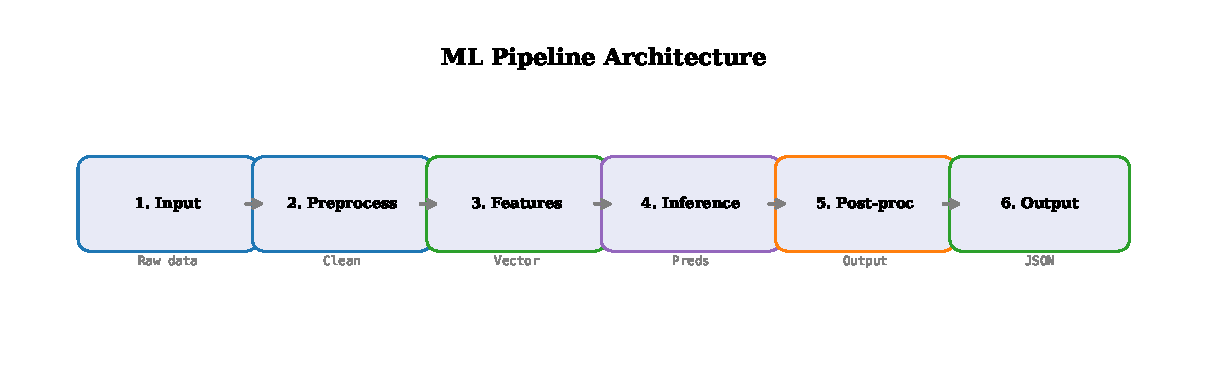
\includegraphics[width=0.85\textwidth]{figures/fig_pipeline_architecture.pdf}
    \caption{Multi-stage pipeline: data flows through sequential processing stages.}
    \label{fig:pipeline-architecture}
\end{figure}

The pipeline architecture enables modular design where each stage is independently testable, replaceable, and upgradeable. If the LLM stage fails, the pipeline continues using the deterministic fallback stage, maintaining system availability.

\subsection{Hybrid Decision Engines}
\label{sec:hybrid-engines}

Hybrid decision engines combine multiple inference paradigms into a unified decision process:

\begin{equation}
\text{decision}(x) = \text{Combine}(f_{\text{rules}}(x), f_{\text{ML}}(x), f_{\text{LLM}}(x))
\label{eq:hybrid-engine}
\end{equation}

where $f_{\text{rules}}$ is the rule engine, $f_{\text{ML}}$ is the ML classifier, and $f_{\text{LLM}}$ is the LLM layer (optional). The combination function uses context-dependent weights (Section~\ref{sec:weighted-blending}) that account for agreement or disagreement between sources.

\begin{figure}[H]
    \centering
    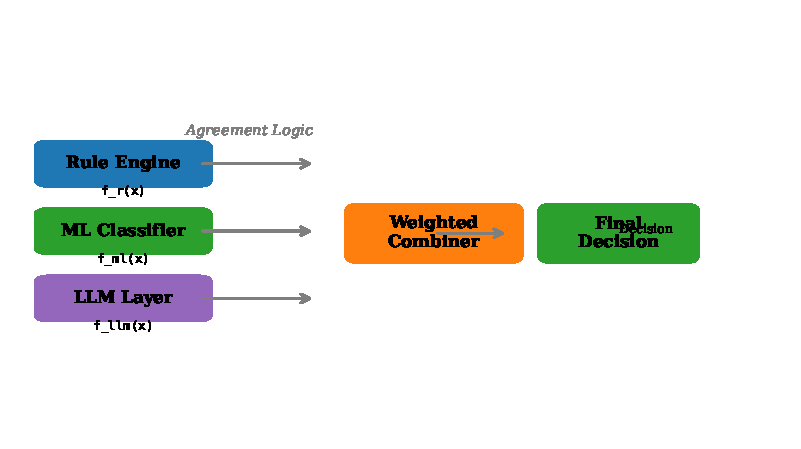
\includegraphics[width=0.85\textwidth]{figures/fig_hybrid_engine.pdf}
    \caption{Hybrid decision engine: rules + ML + LLM combined with weighted score blending.}
    \label{fig:hybrid-engine}
\end{figure}

The hybrid approach achieves higher accuracy and robustness than any single method. Rules handle clear-cut cases with full interpretability, ML captures statistical patterns across thousands of examples, and the LLM interprets semantic nuances in free-text fields. When multiple sources agree, the combined confidence increases; when they disagree, the system routes to manual review.

\subsection{Lazy Loading and Singleton Pattern}
\label{sec:lazy-loading}

Lazy loading defers the initialisation of expensive objects (such as trained ML models and fitted transformers) until they are first needed, rather than at application startup. The Singleton pattern ensures only one instance of a class exists, providing global access to shared resources.

\begin{equation}
\text{LazyLoad}(x) = \begin{cases} \text{existing instance} & \text{if already loaded} \\ \text{load}(\text{path}(x)) & \text{otherwise} \end{cases}
\label{eq:lazy-load}
\end{equation}

Lazy loading reduces application startup time and memory usage when the resource is not always needed. Combined with the Singleton pattern, it ensures that the expensive initialisation (model loading, vocabulary fitting, weight deserialisation) happens exactly once, on first use.

\subsection{Model Serialisation}
\label{sec:model-serialization}

Model serialisation converts trained model objects and fitted transformers into a byte stream for persistent storage:

\begin{equation}
\text{bytes} = \text{serialize}(\{\theta_{\text{model}}, \phi_{\text{transformers}}, \psi_{\text{metadata}}\})
\label{eq:serialization}
\end{equation}

Deserialisation reconstructs the objects from the stored byte stream:

\begin{equation}
\{\theta_{\text{model}}, \phi_{\text{transformers}}, \psi_{\text{metadata}}\} = \text{deserialize}(\text{bytes})
\label{eq:deserialization}
\end{equation}

\begin{figure}[H]
    \centering
    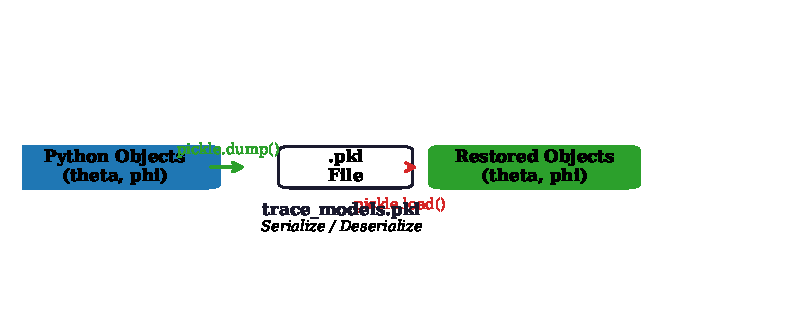
\includegraphics[width=0.85\textwidth]{figures/fig_model_serialization.pdf}
    \caption{Model serialisation: train once, deploy many times.}
    \label{fig:model-serialization}
\end{figure}

Serialisation enables the separation of training and inference phases. Models are trained offline on the full dataset, serialised to a file, and loaded at inference time. This avoids retraining the model on every application restart and ensures that the exact same model (with the same weights and fitted transformers) is used across all inference instances.

\subsection{Auto-Training on Startup}
\label{sec:auto-training}

Auto-training on startup is a resilient system behaviour where the application checks for a persisted model file at startup and automatically trains a new model if none exists:

\begin{equation}
\text{Model} = \begin{cases} \text{load}(\text{MODEL\_PATH}) & \text{if file exists} \\ \text{train\_and\_save}(\text{DATA\_PATH}) & \text{otherwise} \end{cases}
\label{eq:auto-training}
\end{equation}

This pattern ensures the system is always operational, even on first deployment or after a model file is accidentally deleted. In production, pre-trained model files are preferred for faster startup times, but the auto-training fallback provides a safety net that eliminates the need for manual intervention.

% ============================================================
\section{API and Web Architecture}
\label{sec:api-web}

This section covers the web architecture patterns that enable ML model serving, including RESTful API design, data validation, asynchrony, and deployment patterns.

\subsection{RESTful API Design}
\label{sec:rest-api}

Representational State Transfer (REST) is an architectural style for web services that uses standard HTTP methods to perform operations on resources identified by URLs:

\begin{table}[H]
\centering
\caption{HTTP methods and their REST semantics.}
\label{tab:http-methods}
\begin{tabular}{llp{6cm}}
\toprule
\textbf{Method} & \textbf{Action} & \textbf{Semantics} \\
\midrule
GET & Read & Retrieve a resource without side effects \\
POST & Create & Submit data to be processed; create a new resource \\
PUT & Update & Replace an existing resource with new data \\
DELETE & Remove & Delete an existing resource \\
\bottomrule
\end{tabular}
\end{table}

Key principles of RESTful design include statelessness (each request contains all information needed to process it), resource-based URLs (identifying entities, not actions), and standard status codes (200 for success, 400 for client errors, 500 for server errors).

\begin{figure}[H]
    \centering
    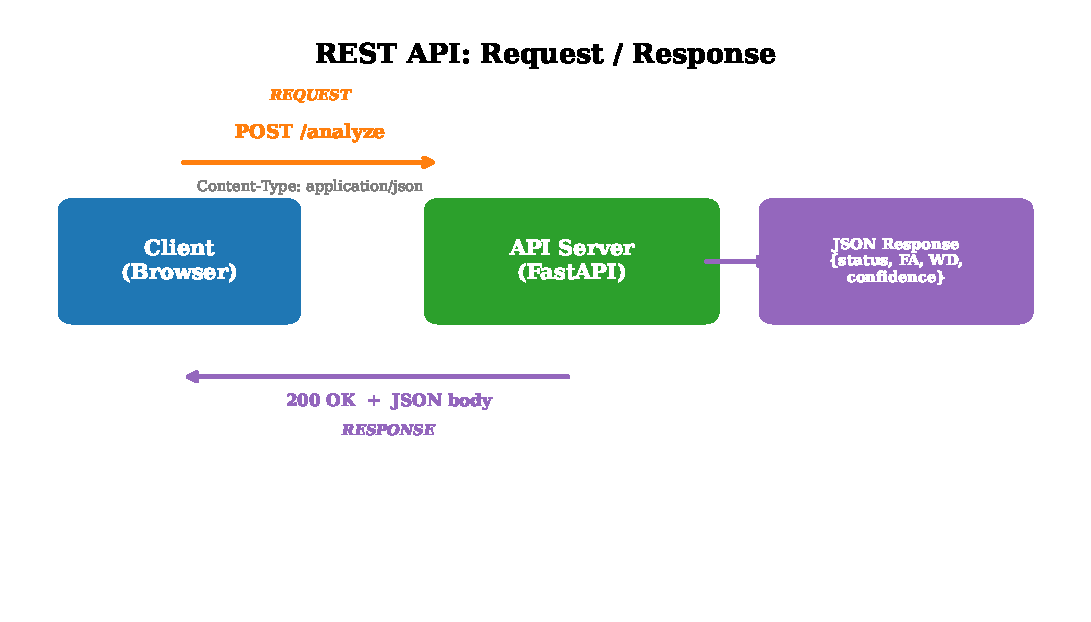
\includegraphics[width=0.85\textwidth]{figures/fig_rest_api.pdf}
    \caption{RESTful API request-response cycle.}
    \label{fig:rest-api}
\end{figure}

\subsection{Pydantic Data Validation}
\label{sec:pydantic}

Pydantic is a Python library that uses type annotations to validate, serialise, and deserialise data at API boundaries. Request schemas are defined as classes inheriting from \texttt{BaseModel}, with each field annotated with its expected type:

\begin{lstlisting}[language=Python]
class ClaimRequest(BaseModel):
    fault_code: str
    technician_notes: str
    voltage: float
\end{lstlisting}

Validation enforces that every incoming request conforms to the declared schema. If a required field is missing or a field has an incorrect type, Pydantic raises a descriptive validation error before the request reaches the ML pipeline:

\begin{equation}
\text{valid}(d) = \begin{cases} \text{true} & \text{if } \forall k, d[k] \text{ matches declared type} \\ \text{false} & \text{otherwise} \end{cases}
\label{eq:pydantic-validation}
\end{equation}

Pydantic prevents malformed input from reaching the prediction engine and provides automatic serialisation of response objects to JSON, ensuring that API responses always conform to the expected schema.

\subsection{CORS Middleware}
\label{sec:cors}

Cross-Origin Resource Sharing (CORS) is a browser security mechanism that controls which external domains can make requests to an API. Without CORS headers, browsers block requests from different origins (protocol + domain + port) for security reasons.

The three key CORS headers are:

\begin{itemize}
    \item \texttt{Access-Control-Allow-Origin}: Specifies which domains may access the API
    \item \texttt{Access-Control-Allow-Methods}: Lists permitted HTTP methods (GET, POST, etc.)
    \item \texttt{Access-Control-Allow-Headers}: Lists permitted request headers
\end{itemize}

CORS middleware adds these headers to every API response, enabling browser-based frontends served from a different origin to communicate with the backend API. In development, a permissive \texttt{allow\_origins=["*"]} setting is common; in production, origins should be restricted to known frontend domains.

\subsection{Async/Await Pattern}
\label{sec:async-await}

The async/await pattern enables a single thread to handle multiple concurrent operations by suspending execution at \texttt{await} points and resuming when the operation completes. For $n$ independent operations with individual durations $t_1, t_2, \ldots, t_n$:

\begin{align}
\text{Synchronous (blocking):} \quad & T_{\text{total}} = \sum_{i=1}^{n} t_i \label{eq:sync-time} \\
\text{Asynchronous (non-blocking):} \quad & T_{\text{total}} = \max(t_1, t_2, \ldots, t_n) \label{eq:async-time}
\end{align}

The async pattern is particularly beneficial for I/O-bound operations such as external API calls (LLM inference), file uploads, and database queries, where the majority of time is spent waiting for a response rather than performing computation. By handling multiple requests concurrently on a single thread, async servers achieve higher throughput without the memory overhead of thread-per-request architectures.

\subsection{HTTP Exception Handling}
\label{sec:http-exceptions}

Structured error handling maps internal exceptions to appropriate HTTP status codes and response bodies:

\begin{table}[H]
\centering
\caption{Common HTTP status codes for API error responses.}
\label{tab:http-errors}
\begin{tabular}{llp{7cm}}
\toprule
\textbf{Code} & \textbf{Name} & \textbf{When to Use} \\
\midrule
400 & Bad Request & Invalid input (missing fields, wrong types) \\
404 & Not Found & Requested resource does not exist \\
422 & Unprocessable Entity & Input is well-formed but semantically invalid \\
500 & Internal Server Error & Unexpected server-side failure \\
\bottomrule
\end{tabular}
\end{table}

Proper error handling provides meaningful error messages to API consumers, distinguishing client errors (4xx) from server errors (5xx). It also logs full exception tracebacks server-side for debugging while returning only user-friendly messages to the client.

\subsection{Environment Variable Configuration}
\label{sec:env-vars}

Environment variables externalise configuration values (API keys, database URLs, feature flags, log levels) from application code, enabling different configurations across environments without code changes:

\begin{itemize}
    \item \textbf{Security:} Secrets (API keys, database passwords) are never stored in source code or version control.
    \item \textbf{Flexibility:} The same code runs in development, staging, and production with different configurations.
    \item \textbf{Containerisation:} Environment variables are injected by container orchestrators at deployment time.
\end{itemize}

Environment variables are typically loaded from a \texttt{.env} file during development and set by the deployment platform in production. A sensible default value should be provided for optional variables to ensure the application can start even when the variable is not set.

\subsection{File Upload and Multipart Form Handling}
\label{sec:file-upload}

HTTP file uploads use the \texttt{multipart/form-data} encoding to transmit binary files alongside metadata in a single request. The multipart format separates each field with a unique boundary string:

\begin{lstlisting}[basicstyle=\ttfamily\small]
--boundary
Content-Disposition: form-data; name="file"; filename="image.jpg"
Content-Type: image/jpeg

[binary data]
--boundary--
\end{lstlisting}

\begin{figure}[H]
    \centering
    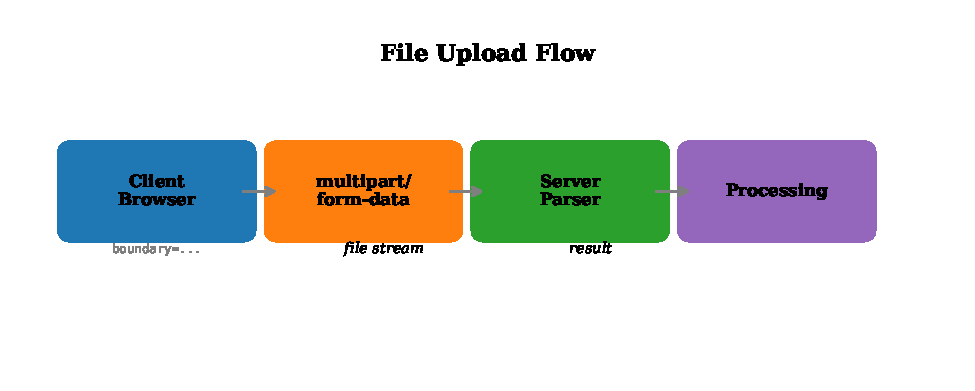
\includegraphics[width=0.85\textwidth]{figures/fig_file_upload_flow.pdf}
    \caption{File upload flow: multipart form data from client to server.}
    \label{fig:file-upload-flow}
\end{figure}

File uploads enable image-based inputs (OCR scanning, document analysis) alongside structured JSON requests. Server-side handlers receive the file as a stream, convert it to an appropriate format (such as a NumPy array for image processing), and pass it to downstream processing stages.

% ============================================================
\section{OCR and Image Processing}
\label{sec:ocr}

Optical Character Recognition (OCR) enables the extraction of structured data from photographs and scanned documents, bridging the gap between visual inputs and machine-readable features.

\subsection{Optical Character Recognition}
\label{sec:ocr-deep-learning}

OCR converts images containing text into machine-readable character strings. Modern deep learning-based OCR systems follow a two-stage pipeline: a detection network locates text regions in the image, and a recognition network decodes the characters within each detected region.

The detection stage produces a set of bounding boxes around text regions in the input image $I$:

\begin{equation}
\text{boxes} = f_{\text{detect}}(I)
\label{eq:ocr-detection}
\end{equation}

The recognition stage then processes each detected region independently:

\begin{equation}
\text{text}_j = f_{\text{recognize}}(I[\text{box}_j])
\label{eq:ocr-recognition}
\end{equation}

The training objective for the recognition stage uses Connectionist Temporal Classification (CTC) loss, which computes the probability of all possible alignments between the input sequence and the output label:

\begin{equation}
L_{\text{CTC}} = -\log \sum_{\pi \in \mathcal{B}^{-1}(y)} \prod_{t=1}^{T} P(\pi_t \mid I)
\label{eq:ctc-loss}
\end{equation}

where $\mathcal{B}^{-1}(y)$ is the set of all CTC paths that collapse to label $y$, and $\pi_t$ is the path token at time step $t$.

\begin{figure}[H]
    \centering
    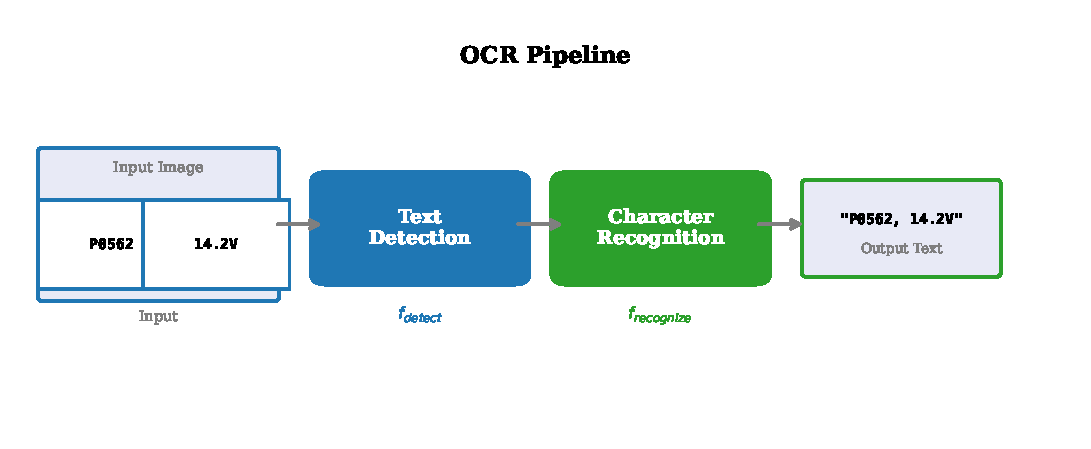
\includegraphics[width=0.85\textwidth]{figures/fig_ocr_pipeline.pdf}
    \caption{Deep learning OCR pipeline: detection then recognition.}
    \label{fig:ocr-pipeline}
\end{figure}

OCR enables the extraction of structured information, such as diagnostic codes and voltage readings, from photographs of diagnostic displays and technician handwritten notes. The accuracy of downstream ML models depends on the quality of OCR output, making post-processing and validation essential.

\subsection{Image-to-Array Conversion}
\label{sec:image-to-array}

Digital images are represented as multidimensional arrays where each element encodes the intensity of a specific pixel and colour channel. An RGB image of dimensions $H \times W$ is stored as a tensor:

\begin{equation}
I \in \mathbb{Z}^{H \times W \times 3}, \quad I_{h,w,c} \in [0, 255]
\label{eq:image-tensor}
\end{equation}

For machine learning processing, pixel values are typically normalised to the $[0, 1]$ range:

\begin{equation}
I_{\text{norm}} = \frac{I}{255.0} \in [0, 1]^{H \times W \times 3}
\label{eq:image-norm}
\end{equation}

This conversion is a standard preprocessing step for any image-based ML pipeline, transforming visual data into a numerical format consumable by neural networks and OCR systems.

\subsection{Structured Data Extraction from Raw Text}
\label{sec:structured-extraction}

Raw OCR output typically contains noise (misread characters, fragmented words, and extraneous symbols). Structured data extraction applies pattern matching and contextual heuristics to identify and isolate specific data fields from the noisy text.

For example, Diagnostic Trouble Codes (DTCs) can be extracted from OCR text using a regular expression:

\begin{equation}
\text{DTCs} = \{s \in \text{OCR}(I) : s \text{ matches } \texttt{\textbackslash b[PUCB][0-9A-Fa-f]\{4\}\textbackslash b}\}
\label{eq:dtc-extraction}
\end{equation}

Voltage values can be extracted by searching for numeric patterns near domain-specific keywords:

\begin{equation}
V = \{v \in \mathbb{R} : v \text{ appears in OCR}(I) \text{ near keyword ``voltage''}\}
\label{eq:voltage-extraction}
\end{equation}

This post-processing step bridges the gap between raw OCR output and structured ML features, handling the inherent noise in photograph-to-text conversion and ensuring that only valid, domain-appropriate values enter the prediction pipeline.

% ============================================================
\section{Logging and Observability}
\label{sec:logging}

Logging and observability provide the mechanisms to monitor, debug, and audit ML system behaviour in production. This section covers the patterns for structured, hierarchical, and domain-specific logging.

\subsection{Centralised Logging Configuration}
\label{sec:centralised-logging}

A centralised logging configuration sets up loggers, handlers, and formatters consistently across an entire application. A \textbf{logger} emits log messages at a specified severity level (DEBUG, INFO, WARNING, ERROR, CRITICAL). A \textbf{handler} directs messages to a destination (console, file, network). A \textbf{formatter} structures each message with metadata such as timestamp, severity, logger name, file name, and line number.

The log format typically follows a structured pattern:

\begin{lstlisting}[language=bash]
%(asctime)s [%(levelname)s] %(name)s %(filename)s:%(funcName)s:%(lineno)d - %(message)s
\end{lstlisting}

This produces log entries such as:

\begin{lstlisting}[language=bash]
2025-01-20 14:32:01 [INFO] trace.ml_predictor ml_predictor.py:predict:845 - INPUT predict | fault_code=P0562 notes_len=42
\end{lstlisting}

\begin{figure}[H]
    \centering
    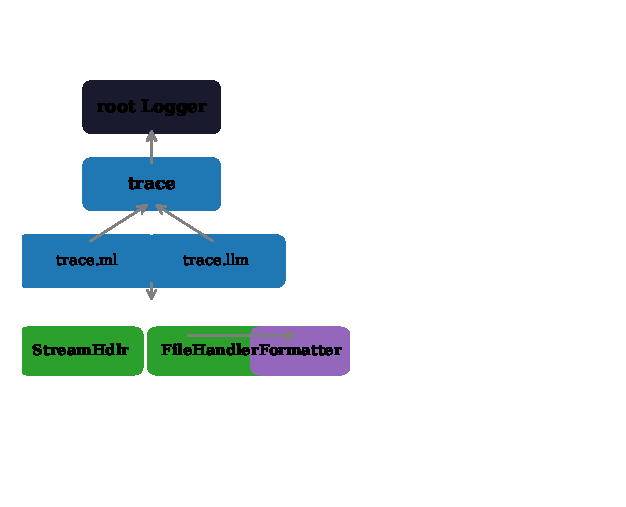
\includegraphics[width=0.85\textwidth]{figures/fig_logging_architecture.pdf}
    \caption{Centralised logging architecture: hierarchical loggers with handlers and formatters.}
    \label{fig:logging-architecture}
\end{figure}

Centralised logging is essential for debugging production ML pipelines, monitoring system health, and maintaining an audit trail of all decisions made by the system.

\subsection{Hierarchical Logger Namespacing}
\label{sec:logger-namespacing}

Hierarchical logger namespacing organises loggers in a dot-separated tree structure (e.g., \texttt{trace.ml\_predictor}, \texttt{trace.llm\_client}, \texttt{trace.api}) that enables selective log level control per module:

\begin{equation}
\text{root} \to \texttt{trace} \to \texttt{trace.ml} \to \texttt{trace.ml.predictor}
\label{eq:logger-hierarchy}
\end{equation}

Child loggers inherit the level of their parent unless explicitly overridden. This allows fine-grained control: for example, setting the ML module to DEBUG level while keeping the API module at INFO level, enabling detailed internal tracing of prediction logic without flooding the logs with routine API request messages.

\subsection{Structured Decision Logging}
\label{sec:decision-logging}

Structured decision logging records the key decisions and intermediate results of each pipeline invocation in a format suitable for automated analysis. A decision log entry typically includes:

\begin{itemize}
    \item Pipeline stage (rule engine, ML classifier, LLM, score combiner)
    \item Input features (fault code, notes length, voltage)
    \item Intermediate outputs (rule fired, ML prediction, LLM category)
    \item Final decision (status, confidence, decision engine tag)
\end{itemize}

Decision logs enable post-hoc analysis of decision patterns, identification of edge cases where the system produces unexpected results, and compliance auditing. They are distinct from general application logs in that they focus on the \emph{why} of each decision, not the \emph{how} of the processing.

% ============================================================
\section{Containerisation and Deployment}
\label{sec:containerisation}

Containerisation packages applications with their dependencies into portable, reproducible execution environments. This section covers the key concepts and patterns for deploying ML systems as containerised services.

\subsection{Docker Containerisation}
\label{section:docker}

Docker packages an application and its dependencies into a lightweight, portable container that runs consistently across different environments. Three key concepts underpin Docker:

\begin{itemize}
    \item \textbf{Image:} A read-only template containing the application code, libraries, runtime, and configuration files needed to run the application.
    \item \textbf{Container:} A running instance of an image with an isolated filesystem, network, and process namespace.
    \item \textbf{Dockerfile:} A text file containing instructions for building an image, including the base image, dependency installation, and application startup command.
\end{itemize}

\begin{figure}[H]
    \centering
    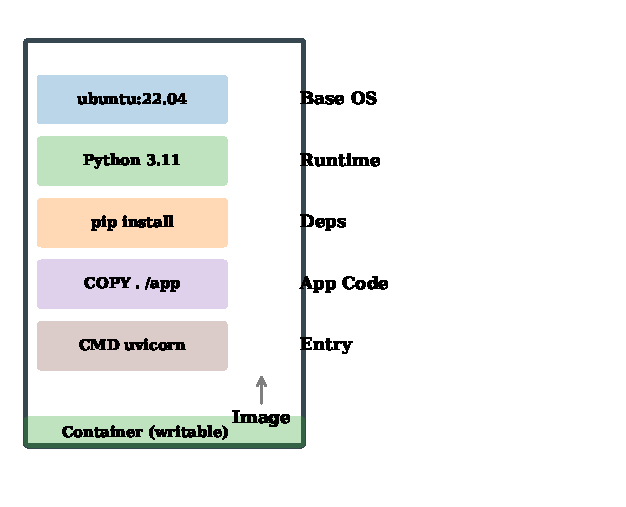
\includegraphics[width=0.85\textwidth]{figures/fig_docker_layers.pdf}
    \caption{Docker image layers: each instruction adds a new layer to the image.}
    \label{fig:docker-layers}
\end{figure}

Docker eliminates ``works on my machine'' problems by ensuring identical runtime environments across development, testing, and production. The layered architecture enables efficient caching: unchanged layers are shared across image builds, reducing build times and storage requirements.

\subsection{Docker Compose Orchestration}
\label{sec:docker-compose}

Docker Compose defines and manages multi-container applications using a single YAML configuration file. It specifies services, networks, and volumes, enabling the entire application stack (API server, frontend, database) to be started with a single command:

\begin{lstlisting}[basicstyle=\ttfamily\small]
services:
  backend:
    build: ./backend
    ports: ["8000:8000"]
    env_file: .env
  frontend:
    build: ./frontend
    ports: ["3000:3000"]
    depends_on:
      backend:
        condition: service_healthy
\end{lstlisting}

Key orchestration features include service dependency management (the frontend waits for the backend health check), network isolation (containers communicate through a shared bridge network), and restart policies (automatic recovery from crashes).

\subsection{Health Checks}
\label{sec:health-checks}

Health checks are automated probes that verify a service is functioning correctly, enabling orchestrators to detect failures and restart unhealthy containers. A health check typically sends an HTTP GET request to a designated endpoint:

\begin{equation}
\text{healthy} = \begin{cases} \text{true} & \text{if HTTP GET } /health \text{ returns 200 within timeout} \\ \text{false} & \text{otherwise} \end{cases}
\label{eq:health-check}
\end{equation}

A restart policy determines when to restart an unhealthy container:

\begin{equation}
\text{restart} = \begin{cases} \text{yes} & \text{if consecutive\_failures} \geq \text{retries} \\ \text{no} & \text{otherwise} \end{cases}
\label{eq:restart-policy}
\end{equation}

\begin{figure}[H]
    \centering
    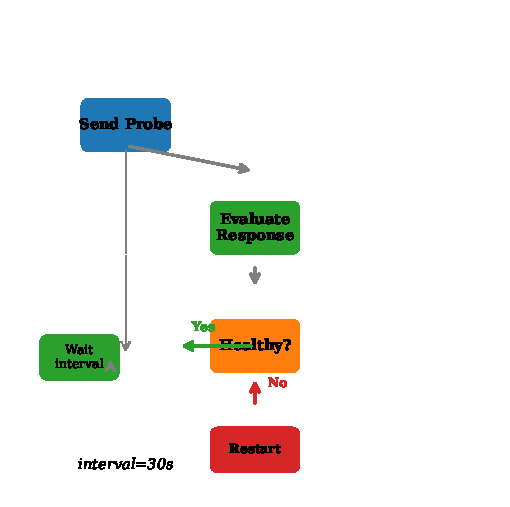
\includegraphics[width=0.85\textwidth]{figures/fig_health_check_cycle.pdf}
    \caption{Health check cycle: probe, evaluate, and restart if unhealthy.}
    \label{fig:health-check-cycle}
\end{figure}

Health checks ensure service reliability by providing automatic recovery from transient failures without manual intervention. They also enable zero-downtime deployments by preventing traffic from being routed to containers that are still initialising.

\subsection{Nginx Static File Serving}
\label{sec:nginx}

Nginx is a high-performance web server and reverse proxy that efficiently serves static files (HTML, CSS, JavaScript) and proxies dynamic API requests to the backend application server. Using Nginx as a reverse proxy separates frontend and backend concerns: Nginx handles static content delivery with minimal overhead, while the application server focuses on business logic and ML inference.

The typical configuration serves the frontend directly and proxies API requests:

\begin{lstlisting}[basicstyle=\ttfamily\small]
location / {
    root /usr/share/nginx/html;
}
location /api/ {
    proxy_pass http://backend:8000;
}
\end{lstlisting}

This pattern provides several benefits: Nginx's event-driven architecture handles static files more efficiently than Python application servers, the reverse proxy adds a layer of security by hiding the backend port, and the frontend and backend can be updated independently.

% ============================================================
\section{Statistical Concepts}
\label{sec:statistics}

This section covers the statistical measures used to validate data quality, assess feature distributions, and verify synthetic data generation.

\subsection{Pearson Correlation}
\label{sec:pearson-correlation}

The Pearson correlation coefficient measures the linear relationship between two continuous variables, ranging from $-1$ (perfect negative correlation) to $+1$ (perfect positive correlation):

\begin{equation}
r_{XY} = \frac{\sum_{i=1}^{n}(x_i - \bar{x})(y_i - \bar{y})}{\sqrt{\sum_{i=1}^{n}(x_i - \bar{x})^2} \sqrt{\sum_{i=1}^{n}(y_i - \bar{y})^2}}
\label{eq:pearson}
\end{equation}

Common thresholds for interpretation are:

\begin{table}[H]
\centering
\caption{Pearson correlation interpretation thresholds.}
\label{tab:correlation-thresholds}
\begin{tabular}{ll}
\toprule
\textbf{Absolute Value} & \textbf{Interpretation} \\
\midrule
$|r| > 0.7$ & Strong correlation \\
$0.3 < |r| \leq 0.7$ & Moderate correlation \\
$|r| \leq 0.3$ & Weak or no correlation \\
\bottomrule
\end{tabular}
\end{table}

\begin{figure}[H]
    \centering
    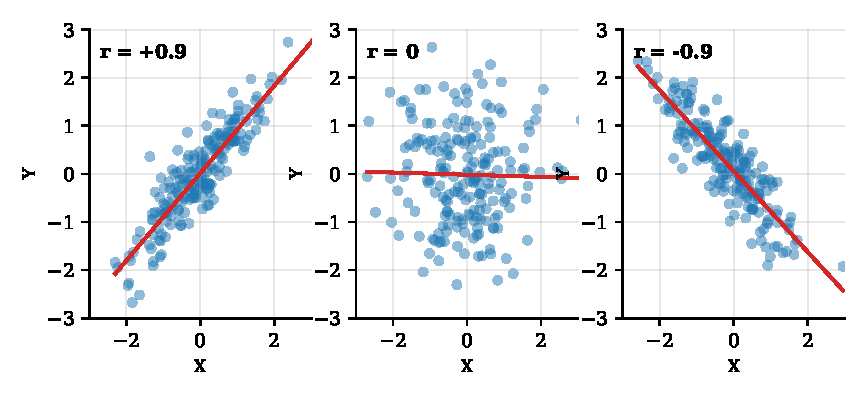
\includegraphics[width=0.85\textwidth]{figures/fig_correlation_scatter.pdf}
    \caption{Pearson correlation: scatter plots for different correlation strengths.}
    \label{fig:correlation-scatter}
\end{figure}

Pearson correlation is used to validate that synthetic data preserves realistic feature relationships and to identify highly correlated features that may introduce multicollinearity in model training.

\subsection{Skewness}
\label{sec:skewness}

Skewness measures the asymmetry of a probability distribution around its mean. Positive skew indicates a right tail (more extreme values above the mean), negative skew indicates a left tail, and zero skew indicates a symmetric distribution.

The sample skewness (Fisher's adjusted) is:

\begin{equation}
g_1 = \frac{\frac{1}{n}\sum_{i=1}^{n}(x_i - \bar{x})^3}{\left(\frac{1}{n}\sum_{i=1}^{n}(x_i - \bar{x})^2\right)^{3/2}}
\label{eq:skewness}
\end{equation}

Interpretation guidelines:

\begin{equation}
g_1 > 0 \text{ (right-skewed)}, \quad g_1 = 0 \text{ (symmetric)}, \quad g_1 < 0 \text{ (left-skewed)}
\label{eq:skewness-interpretation}
\end{equation}

Skewness detection identifies non-normal feature distributions that may require transformation before modelling. For example, mileage data is typically right-skewed because most vehicles have moderate mileage while a few have very high mileage, motivating a log transformation.

\subsection{Kurtosis}
\label{sec:kurtosis}

Kurtosis measures the ``tailedness'' of a distribution, whether it has heavier tails (more outliers) or lighter tails relative to a normal distribution. Excess kurtosis is defined as:

\begin{equation}
\kappa = \frac{\frac{1}{n}\sum_{i=1}^{n}(x_i - \bar{x})^4}{\left(\frac{1}{n}\sum_{i=1}^{n}(x_i - \bar{x})^2\right)^2} - 3
\label{eq:kurtosis}
\end{equation}

The subtraction of 3 makes the normal distribution have excess kurtosis of exactly 0 (mesokurtic). Interpretation:

\begin{equation}
\kappa > 0 \text{ (leptokurtic, heavy tails)}, \quad \kappa = 0 \text{ (mesokurtic, normal)}, \quad \kappa < 0 \text{ (platykurtic, light tails)}
\label{eq:kurtosis-interpretation}
\end{equation}

Leptokurtic distributions ($\kappa > 0$) have more extreme outliers than the normal distribution, which can affect model robustness. Identifying high-kurtosis features helps anticipate potential issues with outliers and informs the choice of robust statistical methods.

\subsection{Quantile Analysis}
\label{sec:quantile-analysis}

Quantile analysis divides a dataset into equal-sized groups based on value rank, enabling analysis of distribution characteristics beyond mean and variance. The $q$-th quantile is defined as:

\begin{equation}
Q(q) = \inf\{x : F(x) \geq q\}, \quad q \in (0, 1)
\label{eq:quantile}
\end{equation}

where $F(x)$ is the empirical cumulative distribution function. The interquartile range (IQR) measures the spread of the middle 50\% of the data:

\begin{equation}
\text{IQR} = Q(0.75) - Q(0.25)
\label{eq:iqr}
\end{equation}

The IQR-based outlier detection rule identifies observations that fall more than 1.5 IQR below the first quartile or above the third quartile:

\begin{equation}
\text{outlier} = x \text{ if } x < Q(0.25) - 1.5 \cdot \text{IQR} \text{ or } x > Q(0.75) + 1.5 \cdot \text{IQR}
\label{eq:iqr-outlier}
\end{equation}

\begin{figure}[H]
    \centering
    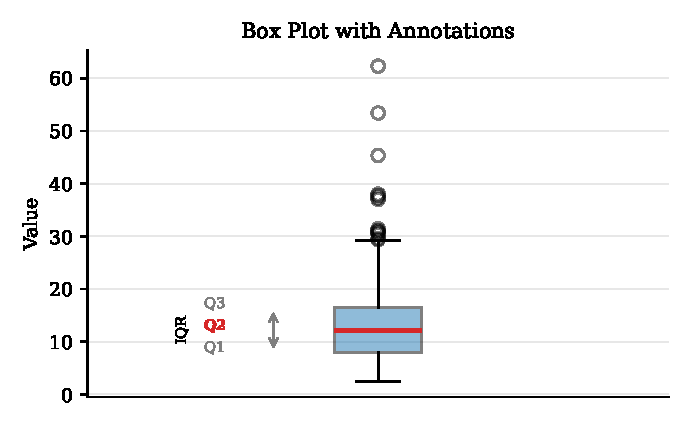
\includegraphics[width=0.8\textwidth]{figures/fig_box_plot.pdf}
    \caption{Box plot: median, quartiles, IQR, and outliers identified by the 1.5 IQR rule.}
    \label{fig:box-plot}
\end{figure}

Quantile analysis provides robust feature statistics that are not influenced by extreme outliers, unlike mean and standard deviation. It also enables quantile-based binning, which captures domain-relevant thresholds directly from the data distribution.

\end{document}